\documentclass[10pt]{article}

\usepackage{amsmath,amsthm,amssymb,xcolor,graphicx,tikz,listings}
\usepackage{comment}
\usepackage{cite}
\usepackage[T1]{fontenc}
\usepackage[utf8x]{inputenc}
\usepackage[pdftex]{hyperref}
\usetikzlibrary{positioning}

\begin{document}

% Macros
%------------------------------------------------------------
\def\Any {{\mathcal U}}
\def\Prop{{\mathcal P}}
\def\Indsort{{\Any_\mathcal I}}
\def\Fixsort{{\Any_\mathcal F}}
\def\Uni {{\mathcal L}}
\def\Univ {{\mathcal L}}
\def\Top {{\Box}}

\def\Nat{{\mathbb N}}

\def\case{{\text{\it case}}}
\def\ctree{{\text{\it tree}}}
\def\ct#1{{\mathcal #1}}
\def\cta {{\text{cta}}}
\def\fix {{\text{\it fix}}}
\def\fspinetree{{f_\text{st}}}
\def\llet{{\text{\it let}}}
\def\type{{\text{\it type}}}
\def\FV  {{\text{\it FV}}}

\def\Ind{{\cal I}}
\def\Make{{\cal M}}

\def\empty {\varepsilon}
\def\reduce{\leadsto}
\def\genreduce#1{\,\stackrel{#1}{\leadsto}\,}
\def\hreduce{\genreduce h}
\def\hstarreduce{\genreduce h^*}
\def\equiv {\,\sim\,}

%\def\meta#1{{{}^?\!\!#1}}
\def\meta#1{{{}^? \kern-0.2em #1}}
%\def\meta#1{{? \kern-0.2em #1}}
%\def\meta#1{{#1_?}}


\def\impl{\rightarrow}
%\def\vec#1{{\mathbf #1}}
\def\vec#1{{\overrightarrow {#1}}}
\def\fargs#1#2{{\vec {#1}^{\vec {#2}}}}

\def\set#1{{\{#1\}}}

\def\betaeq{{\stackrel \beta \sim}}


\def\brackets#1{\left[ {#1} \right]}
\def\parens#1{\left( {#1} \right)}

\def\ctreebr#1{{\ctree \brackets {#1}}}
\def\letbr#1{{\llet \brackets {#1}}}
\def\fixbr#1{{\fix  \brackets {#1}}}

\def\vertlist#1{
    \begin{array}{lllll}
    #1
    \end{array}
}

\def\bracklist#1{\brackets{ \vertlist{#1} }}


\def\cases#1{
    \left\{ \vertlist {#1} \right.
}


\def\rulev#1#2{
    \begin{array}{l}
        #1
        \\
        \hline
        #2
    \end{array}
}

\def\ruleh#1#2{
    \begin{array}{c}
        #1
        \\
        \hline
        #2
    \end{array}
}




% Put description label in italic (and not in bold)
\renewcommand{\descriptionlabel}[1]{\hspace{\labelsep}\textit{#1}}



\title{
    Compiling Alba
}

\author{
    Helmut Brandl
    \\
    \scriptsize (firstname dot lastname at gmx dot net)
}
\date{}

\maketitle


\abstract{
    How to compile Alba programs.
}


\tableofcontents

% Macros
%------------------------------------------------------------
\def\Any {{\mathcal U}}
\def\Prop{{\mathcal P}}
\def\Indsort{{\Any_\mathcal I}}
\def\Fixsort{{\Any_\mathcal F}}
\def\Uni {{\mathcal L}}
\def\Univ {{\mathcal L}}
\def\Top {{\Box}}

\def\Nat{{\mathbb N}}

\def\case{{\text{\it case}}}
\def\ctree{{\text{\it tree}}}
\def\ct#1{{\mathcal #1}}
\def\cta {{\text{cta}}}
\def\fix {{\text{\it fix}}}
\def\fspinetree{{f_\text{st}}}
\def\llet{{\text{\it let}}}
\def\type{{\text{\it type}}}
\def\FV  {{\text{\it FV}}}

\def\Ind{{\cal I}}
\def\Make{{\cal M}}

\def\empty {\varepsilon}
\def\reduce{\leadsto}
\def\genreduce#1{\,\stackrel{#1}{\leadsto}\,}
\def\hreduce{\genreduce h}
\def\hstarreduce{\genreduce h^*}
\def\equiv {\,\sim\,}

%\def\meta#1{{{}^?\!\!#1}}
\def\meta#1{{{}^? \kern-0.2em #1}}
%\def\meta#1{{? \kern-0.2em #1}}
%\def\meta#1{{#1_?}}


\def\impl{\rightarrow}
%\def\vec#1{{\mathbf #1}}
\def\vec#1{{\overrightarrow {#1}}}
\def\fargs#1#2{{\vec {#1}^{\vec {#2}}}}

\def\set#1{{\{#1\}}}

\def\betaeq{{\stackrel \beta \sim}}


\def\brackets#1{\left[ {#1} \right]}
\def\parens#1{\left( {#1} \right)}

\def\ctreebr#1{{\ctree \brackets {#1}}}
\def\letbr#1{{\llet \brackets {#1}}}
\def\fixbr#1{{\fix  \brackets {#1}}}

\def\vertlist#1{
    \begin{array}{lllll}
    #1
    \end{array}
}

\def\bracklist#1{\brackets{ \vertlist{#1} }}


\def\cases#1{
    \left\{ \vertlist {#1} \right.
}


\def\rulev#1#2{
    \begin{array}{l}
        #1
        \\
        \hline
        #2
    \end{array}
}

\def\ruleh#1#2{
    \begin{array}{c}
        #1
        \\
        \hline
        #2
    \end{array}
}




% Put description label in italic (and not in bold)
\renewcommand{\descriptionlabel}[1]{\hspace{\labelsep}\textit{#1}}


\lstdefinelanguage{alba}
{ basewidth=0.45em,
  basicstyle=\scriptsize\tt,  % choices: small, footnotesize, scriptsize, tiny
  mathescape,
  %columns=flexible,
  keywords={
    abstract,all,and,
    case,
    do,
    else,end
    ghost,
    if,in,inspect,
    let,
    mod,
    mutual,
    not,
    or,
    record,
    section,some,
    then,
    type,
    use,
    where,
    And,
    Not,
    Or
  },
  keywordstyle=\color{blue},
  commentstyle=\color{brown},
  morecomment=[l]{--},
  morecomment=[n]{\{-}{-\}}
}

\lstnewenvironment{alba} {\lstset{language=alba}} {}


\lstset{language=alba}

\section{Calculus}





\subsection{Terms and Contexts}
%--------------------------------------------------------------------------------



The terms are generated by the grammar
%
$$
\begin{array}{llll}
    t
    &::=&
    \Prop
    &\text{propositional sort}
    \\
    &\mid&
    \Any
    &\text{computational sort}
    \\
    &\mid&
    c
    &\text{constants (numbers, strings, $\ldots$)}
    \\
    &\mid&
    x
    &\text{variables}
    \\
    &\mid&
    \meta m
    &\text{metavariables}
    \\
    &\mid&
    \type_i\brackets{\Gamma \mid \vec {I^K := \vec C}}
    & \text{inductive types}
    \\
    &\mid&
    \Make^{\mathcal I}_{\ell_i}
    &\text{constructors}
    \\
    &\mid&
    f \vec a
    & \text{application}
    \\
    &\mid&
    \lambda \vec {x^A}. e
    & \text{abstractions}
    \\
    &\mid&
    \Pi \vec {x^A}. R
    & \text{products}
    \\
    &\mid&
    \fix_i\brackets{\Gamma \mid \vec{ f^F := e}}
    & \text{fixpoints}
    \\
    &\mid&
    \llet\brackets{\vec{ x^A := \vec a} \mid e}
    & \text{let expressions}
    \\
    &\mid&
    \case[f^F \mid \vec c \mid t]
    & \text{case expressions}
    \\
    &\mid&
    \cta[f, t, \vec u, p]
    &\text{case tree application}
\end{array}
$$
%
and contexts are generated by the grammar
$$
\begin{array}{llll}
    \Gamma
    &::=&
    []
    &\text{empty context}
    \\
    &\mid&
    \Gamma, x^A
    &\text{local variable}
    \\
    &\mid&
    \Gamma, (x^A := a)
    &\text{definition}
    \\
    &\mid&
    \Gamma, \meta m^M
    &\text{meta variable}
    \\
    &\mid&
    \Gamma, (\meta m^M := a)
    &\text{meta variable instantiation}
\end{array}
$$






\subsection{Head Reductions}
%--------------------------------------------------------------------------------

The following head reductions are possible:
$$
\begin{array}{llll}
        \Gamma \vdash (\lambda \vec x^{\vec A}. e) \vec a \vec b
        &\hreduce&
        \Gamma, [\vec x^{\vec A} := \vec a] \vdash e \vec b
        \\
        \Gamma \vdash \llet[\vec x^{\vec A} := \vec a , e] \vec b
        &\hreduce&
        \Gamma, [\vec x^{\vec A} := \vec a] \vdash e \vec b
        \\
        \Gamma \vdash \case[*, *, t] \vec a \vec b
        &\hreduce&
        \Gamma \vdash \cta[\case[*,*,t], t, \empty, p.f = a_1] \vec b
        \\
        \Gamma \vdash \cta[*, t_1, \vec u_1, p_1] \vec b
        &\hreduce&
        \Gamma \vdash \cta[*, t_2, \vec u_2, p_2] \vec b
        \\
        \Gamma
        \vdash
        \cta(\text{pm}, e, \vec u, \empty) \vec b
        %
        &\hreduce&
        %
        \Gamma, [f,\vec x := \text{pm}, \vec u]
        \vdash
        e \vec b
        \\
        \\
        \Gamma \vdash x \vec b
        &\hreduce&
        \Gamma \vdash a \vec b
\end{array}
$$

The last reduction is an unfolding of a definition i.e. $(x:=a) \in \Gamma$ is
assumed. A case tree application can become stuck if the focal term does not
allow a decision.

Note that the head reductions only make substitutions of head terms. Instead of
substitutions variables with definitions are introduced.






\subsection{Typing Rules}
%--------------------------------------------------------------------------------

We introduce two relations.
$$
\Gamma \vdash t: T
$$
Read: In the context $\Gamma$ the term $t$ has type $T$.
$$
\Gamma \vdash A \le B
$$
Read: $A$ and $B$ are welltyped in the context $\Gamma$ and $A$ is a subtype of
$B$.





The rules for $\Gamma \vdash t : T$:

$$
\vertlist {
    \text{axiom} &
    %----------------
    [] \vdash \Prop: \Any_0
    \quad
    \rulev{
        i < j
    }
    {
        [] \vdash \Any_i : \Any_j
    }
    \\
    \\
    \text{var add} &
    %----------------
    \rulev{
        \Gamma \vdash A: s
    }
    {
        \Gamma, x^A \vdash x: A
    }
    \quad
    \rulev{
        \Gamma \vdash a: A
    }
    {
        \Gamma, [x^A := a] \vdash x: A
    }
    \\
    \\
    \text{def elim} &
    %----------------
    \rulev{
        \Gamma, [x^A:= a] \vdash t : T
    }
    {
        \Gamma \vdash t[a/x] : T[a/x]
    }
    \quad
    \rulev{
        \Gamma, [x^A:= a] \vdash t : T
    }
    {
        \Gamma, x^A \vdash t : T
    }
    \\
    \\
    \text{product} &
    %----------------
    \rulev{
        \Gamma \vdash A: s
        \\
        \Gamma, x^A \vdash B: \Prop
    }
    {
        \Gamma \vdash \Pi x^A. B: \Prop
    }
    \quad
    \rulev{
        \Gamma \vdash A: \Any_i
        \\
        \Gamma, x^A \vdash B: \Any_j
    }
    {
        \Gamma \vdash \Pi x^A. B: \Any_{\text{max}(i,j)}
    }
    \\
    \\
    \text{pi elim} &
    %----------------
    \rulev{
        \Gamma,[x^A:=a],\Delta \vdash \Pi x^A. B
    }
    {
        \Gamma,[x^A:=a],\Delta \vdash B
    }
    \\
    \\
    \text{lambda} &
    %----------------
    \rulev{
        \Gamma, x^A \vdash e : B
    }
    {
        \Gamma \vdash \lambda x^A. e := \Pi x^A. B
    }
    \\
    \\
    \text{app} &
    %----------------
    \rulev{
        \Gamma, [x^A:=a], \Delta \vdash f : \Pi x^A. B
    }
    {
        \Gamma, [x^A := a], \Delta \vdash f x: B
    }
    \\
    \\
    \text{weaken} &
    %----------------
    \rulev{
        \Gamma \vdash t: T
        \\
        \Gamma \vdash A: s
    }
    {
        \Gamma, x^A \vdash t : T
    }
    \quad
    \rulev{
        \Gamma \vdash t: T
        \\
        \Gamma \vdash a: A
    }
    {
        \Gamma, [x^A:=a] \vdash t : T
    }
    \\
    \\
    \text{subtype} &
    %----------------
    \rulev{
        \Gamma \vdash t : T
        \\
        \Gamma \vdash T \le U
    }
    {
        \Gamma \vdash t: U
    }
}
$$


The rules for $\Gamma \vdash A \le B$:
$$
\vertlist {
    \text{axiom} &
    %---------------
    [] \vdash \Prop \le \Any_0
    \quad
    \rulev {
        i \le j
    }
    {
        [] \vdash \Any_i \le \Any_j
    }
    \\
    \\
    \text{product} &
    %---------------
    \rulev {
        \Gamma \vdash A_2 \le A_1
        \\
        \Gamma, x^{A_2} \vdash B_1 \le B_2
    }
    {
        \Gamma \vdash \Pi x^{A_1}.B_1 \le \Pi x^{A_2}. B_2
    }
    \\
    \\
    \text{inductive} &
    %---------------
    \text{MISSING}
    \\
    \\
    \text{weaken} &
    %---------------
    \rulev {
        \Gamma \vdash T \le U
        \\
        \Gamma \vdash A : s
    }
    {
        \Gamma, x^A \vdash T \le U
    }
    \quad
    \rulev {
        \Gamma \vdash T \le U
        \\
        \Gamma \vdash a: A
    }
    {
        \Gamma, [x^A := a] \vdash T \le U
    }
    \\
    \\
    \text{unfold} &
    %---------------
    \rulev {
        \Gamma \vdash a : A
        \\
        \Gamma,[x^A:=a],\Delta \vdash T \le U
    }
    {
        \Gamma,\Delta[a/x] \vdash T[a/x] \le U[a/x]
    }
    \\
    \\
    \text{same} &
    %---------------
    \rulev {
        \Gamma \vdash A: s
    }
    {
        \Gamma \vdash A \le A
    }
    \\
    \\
    \text{equiv} &
    %---------------
    \rulev {
        \Gamma \vdash A \equiv B
        \\
        \Gamma \vdash B \le C
        \\
        \Gamma \vdash C \equiv D
    }
    {
        \Gamma \vdash A \le D
    }
}
$$


\section {Inductive Types}


\subsection{Form of an inductive type:}
%--------------------------------------------------------------------------------


$$
    \type_i[\Gamma, \vec {X^K := \vec C}]
$$

\begin{description}
    \item [Parameters $\Gamma$] Context of parameters. It binds all free
        variables in the kinds and the constructurs.

    \item [Kinds $K_i$] The have the form $\Pi \vec {x^A}. s$ of a function
        type.
        Kinds have an arity which is possibly zero and a sort $s$ as its
        result type.

    \item [Constructor types $C_{i \ell_j}$] Each constructor type has a label.
        All labels for the same $i$ must be different. The constructor types
        have the form
        $$
            \Pi \Delta. X_i \vec a
        $$
        where the context $\Delta$ might be empty and all $X_j$ can occur in
        $\Delta$ only positively i.e. $\Delta$ has the structure
        $$
            [y_1^{\Pi B_1. R_1}, \ldots, y_n^{\Pi B_m. R_m}]
        $$
        and $X_j$ can occur only in $R_i$ and if it occurs in $R_i$, then $R_i$
        has the form $X_j \vec a$. I.e. the arguments of constructors are
        functions (arity zero included) where $X_j$ occurs only in the result type
        and not in the argument types.

    \item [Recursive]
        An inductive type is recursively defined if $X_j$ occurs in the result
        type of any constructor argument.
\end{description}


\begin{alba}
    type Nat: Any :=
        zero: Nat
        succ: Nat -> Nat


    type (<=): Nat -> Nat -> Prop
    :=
        z<=n {n}: zero <= n
        s<=s {n m}: n <= m -> succ n <= succ m


    mutual (A: Any)
        type Tree: Any :=
            node: A -> Forest -> Tree

        type Forest: Any :=
            []: Forest
            (::): Tree -> Forest -> Forest


    type Acc {A: Any} (R: A -> A -> Prop): A -> Acc
    :=
        acc {x}: (all {y}: R y x -> Acc y) -> Acc x


    type (=) {A: Any}: A -> A -> Prop
    :=
        refl {x}: x = x
\end{alba}


\paragraph{Implementation Hints}
\begin{enumerate}
    \item Since the result type of a constructor must always have the form $X
        \vec a$ it is not necessary to store the whole expression. It is
        sufficient to store the index arguments $\vec a$.

        \begin{alba}
            type Nat: Any :=
                zero: _
                succ: Nat -> _

            type (<=): Nat -> Nat -> Prop
            :=
                z<=n {n}: _ zero n
                s<=s {n m}: n <= m -> _ (succ n) (succ n)
        \end{alba}

    \item The kinds must have the form $\Pi \vec{x^A}. s$. It is sufficient to
        store the array of the index arguments $\vec {x^A}$ and the sort.

    \item The constructor types have the form $\Pi \vec{y^D}. X_i \vec a$. The
        constructor arguments $\vec {y^D}$ can be stored as an array (i.e. a
        context). If any $X_j$ occurs in a type of a constructor argument
        (recursive case), then
        it can occur only as a result type. The non recursive argument types can
        be stored just as a normal term. The recursive argument types can be
        stored as an array plus the result type.

    \item Parameters of type $\Prop$ or $\Any$ can generate nested inductive
        types (e.g. {\tt List (Tree A)}). Therefore it might be interesting to
        check, if a type variable occurs only positively in constructor
        arguments.
\end{enumerate}




\subsection{Examples}
%--------------------------------------------------------------------------------
$$
    \begin{array}{lll}
        \text{boolean}
        &
        \type[B^\Any \mid B, B]
        \\
        %
        \text{peano numbers}
        &
        \type[N^\Any \mid N, N\to N]
        \\
        %
        \text{list}
        &
        \type[A^\Any \mid L^\Any \mid L, A \to L\to L]
        \\
        %
        \text{equality}
        &
        \type[A^\Any
        \mid E^{A \to A \to \Prop}
        \mid \Pi x^A. E x x]
        \\
        %
        \text{accessibles}
        &
        \type[
            A^\Any, R^{A \to A \to \Prop}
            \mid
            T^{A \to \Prop}
            \mid
            \Pi x^A. (\Pi y^A. R y x \to T y) \to T x
        ]
    \end{array}
$$

In peano numbers the first constructor type has no arguments. The second has one
recursive argument.




\subsection{Constructors}
%--------------------------------------------------------------------------------

$$
    \Make^\Ind_{\ell_i} \vec p \vec b: \Ind \vec p \vec a
$$
where $\Ind$ is the inductive type, $i$ marks the $i$th constructor, $\vec p$ are
the parameter arguments and $\vec b$ are the constructor arguments, $a$ are the
index arguments which depend on the constructor arguments.

The peano number $2$ looks like $ \Make^N_1 (\Make^N_1 \Make^N_0) $.

A constructor has the type
$$
    \Make^\Ind_{\ell_i} : \Pi \Gamma \Delta_{\ell_i}. T {\vec a}_{\ell_i}
$$





\subsection{Typing}
%--------------------------------------------------------------------------------

Let $\Ind = [\Gamma \mid T^K \mid C_{\ell_1}, \ldots, C_{\ell_n}]$ be a wellformed
inductive type. Then we have the following typing rules.

\begin{description}

    \item [Inductive type]
        $$
            \rulev{
                K \; \betaeq\; \Pi \Gamma_K. s
                \\
                \forall i.\; \Gamma, T^K \vdash C_{\ell_i}: s
            }
            {
                [] \vdash \Ind : \Pi \Gamma. K
            }
        $$


    \item [Constructor] Let $C_{\ell_i} = \Pi \Delta. T \vec a$.
        $$
        \rulev{
            [] \vdash \Ind: \Pi \Gamma. K
        }
        {
            \Make^\Ind_{\ell_i}: \Gamma \Delta.T \vec a
        }
        $$
\end{description}






\subsection{Mutually defined Inductive Types}
%--------------------------------------------------------------------------------

It is just an array of inductive types where all inductive types share the same
parameters.
$$
    \type
    \left[\Gamma \mid
    \bracklist{
        T_1^{K_1} \mid C_{11}, \ldots, C_{1n_1}
        \\
        \ldots
        \\
        T_m^{K_m} \mid C_{m1}, \ldots, C_{mn_m}
    }
    \right]
$$

All kinds $K_i$ are valid in the context $\Gamma$ and all constructors of the
$i$th type construct an object of type $T_i \vec a$ but can use any other
objects of type $T_j \vec a$ as arguments. All constructors are valid types in
the context $\Gamma, T_1^{K_1}, \ldots , T_m^{K_m}$.


\section{Pattern Match}
%----------------------------------------------------------------------

\subsection{Basics}
%----------------------------------------------------------------------

Fully elaborated pattern match expression:
$$
\case[ f^F \mid c_1,  \ldots, c_n \mid t]
$$
%
where $F$ is a function type of the form
%
$$
\Pi x_1^{A_1} \ldots x_k^{A_k}. R
$$
%
and where each clause $c_i$ has the form
%
$$
    [\Delta \mid p_1^{P_1}, \ldots, p_m^{P_m} \mid e^E]
$$
where the context $\Delta$ contains all pattern variables introduced in the
pattern, $p_i$ is the $i$-th pattern
and $P_i$ is the corresponding type of the pattern, $e$ is the body of the
clause, $E$ its corresponding type and $t$ is a case tree (see below).

Each clause defines the function
$$
\lambda \Delta . e^E
$$


The patterns are terms generated from the grammar
$$
    p ::= x \mid x := c \mid x := \Make^I_\ell \vec q \vec p
$$
where $c$ ranges over constants (strings, characters, numbers, etc.), $x$ ranges
over variables and $p$ ranges over pattern. The expression $\Make^I_\ell \vec q
\vec p$ is the constructor with label $\ell$ of the inductive type $I$ applied to its
parameter arguments and to its arguments.

Patterns are trees. Each node of the tree is labelled by a pattern variable and
either by a constant or a constructor $\Make^I_\ell \vec q$. A pattern clause has a
sequence of trees.

The pattern variables are assumed to be distinct in all clauses.



\subsection{Welltyped}
%------------------------------------------------------------

A clause of the pattern match expression is welltyped if
$$
\begin{array}{lll}
    \Delta &\vdash& p_i : P_i
    \\
    \Delta &\vdash& e : E
\end{array}
$$
%
and
%
$$
\begin{array}{lll}
    P_i &\le& A_i[p_1,\ldots,p_{i-1} / x_1,\ldots,x_{i-1}]
    \\
    E   &\le& R[p_1,\ldots,p_m / x_1,\ldots,x_m]
\end{array}
$$
%
where $F = \Pi x_1^{A_1} \ldots x_m^{A_m}. R$.




\subsection{Syntactical Pattern}
%------------------------------------------------------------

The pattern in the source code are generated from the grammar
$$
\begin{array}{llll}
    p_s
    &:=&   x                   & \text{pattern variable}
    \\
    &\mid& \ell \vec p_s       & \text{constructor + arguments}
    \\
    &\mid& c                   & \text{constant}
    \\
    &\mid& x := \ell \vec p_s
    \\
    &\mid& x := c
\end{array}
$$


A constructor label $\ell$ without arguments and a variable name $x$ are
indistiguishable in the source code. They are just names. But since the required
type is known it is clear if the name is one of the labels of the corresponding
inductive type. In that case the name is a label and not a pattern variable.






\subsection{Case Tree}
%------------------------------------------------------------

A case expression is a function which can be applied to arguments
$$
    \case[\ldots] a_1 \ldots a_n
$$
%
The task of a valid case tree is to
\begin{itemize}
    \item split the arguments into a series of subterms $u_1,u_2, \ldots$

    \item decide which case clause is applicable (if sufficient information is
        available)

    \item return the result $e[u_1, u_2, \ldots / .]$ where $e$ is the right
        hand side of the applicable case clause.
\end{itemize}

A case tree is defined by the grammar

$$
    \begin{array}{lllll}
        t
        &::=& e
        %
        \\
        &\mid& [x^T \mid t]
        %
        \\
        &\mid& [
            x^T
            \mid
            c_1 t_1, \ldots,  c_n t_n \mid
            \ell_1 t_1, \ldots, \ell_m t_m
            \mid
            d
        ]
    \end{array}
$$
%
where $n + m > 0$ and
%
\begin{center}
    \begin{tabular}{l p{8cm}}
        $t$ & case tree
        \\
        $d$ & optional case tree (default or catch all)
        \\
        $e$ & expression on the right hand side of a case clause
        \\
        $x^T$ & pattern variable with its corresponding type
        \\
        $c$ & constant
        \\
        $\ell$ & label of a constructor
    \end{tabular}
\end{center}

We can abbreviate the second form of an inner node by $[x^T \mid \vec c\vec t \mid
\vec\ell \vec t | d]$.


No duplicate constants and no duplicate labels are allowed in the second form of
an inner node.

The application of a case scans the list of arguments left to write with a
pointer to a subexpression to some of its arguments. Semantic actions associated
to the nodes of a case tree.
\begin{itemize}
    \item $e$: The pointer has to point beyond the last argument of the
        arguments. The list of collected subexpression $u_1, u_2, \ldots$ cover
        all free variables in the expression $e$. Action: Return the value
        $e[u_1,u_2,\ldots / .]$.

    \item $[x^T \mid t]$: The pointer has to point to some subexpression of the
        arguments and there has to be a next pointer position. Action: Append
        the term $u$ to the list of terms $u_1,u_2,\ldots$ where $u$ is the
        subexpression at the pointer and apply the case tree $t$ to the pointer
        advance by one.

    \item $[x^T \mid \vec c \vec t \mid \vec \ell \vec t \mid d]$:
        The pointer has to point to some subexpression of the arguments. The
        subexpression has to reduce to a head normal form which has either a
        constant or a constructor in the head position. From the constant or the
        constructor it is clear which case tree is the next to apply.
        Actions:
        \begin{itemize}
            \item Append the subexpression to the list $u_1,u_2,\ldots$.

            \item If the default tree is the next tree then apply it to the next
                pointer position.

            \item If the subexpression is a constant then apply the
                corresponding next tree to the next pointer position.

            \item If the subexpression is a constructor without index
                arguments then apply the corresponding next tree to the next
                pointer position.

            \item If the subexpression is a constructor with arguments then
                apply the corresponding next tree to the pointer pointing at the
                first index argument of the constructor (skip the parameter
                arguments).
        \end{itemize}
\end{itemize}



\paragraph{Exhaustiveness of inner nodes}
%

An inner node of the form $[x^T \mid \vec c \vec t \mid \vec\ell \vec t \mid d]$ is
exhaustive if it has a default tree or if all labels of constructors which can
construct an object of the corresponding type are present (none of the missing
constructors can construct an object of type $T$).

An empty inner node of the form $[x^T \mid \empty \mid \empty \mid \empty]$ is
possible if $T$ is an inductive type and none of the constructors of the
inductive type can construct an object of type $T$.

\paragraph{Exhaustiveness of a case tree}
%
A case tree is exhaustive if all its nodes are exhaustive.



\paragraph{Redundancy of an inner node}

An inner node of the form $[x^T \mid \vec c \vec t \mid \vec\ell \vec t \mid d]$
is redundant if
\begin{itemize}
    \item it has multiple entries of the same constant

    \item it has multiple entries of the same constructor

    \item it has a default tree and none of the missing constructors can
        construct an object of type $T$ or there are no missing constructors.
\end{itemize}



\paragraph{Redundancy of case tree}

A case tree is redundant of some of its nodes are redundant.




\subsection{Case Tree Construction}
%------------------------------------------------------------

\paragraph{Case tree for a clause}
First we construct a case tree from a cause clause
$\Delta \vec p^{\Vec p} := e$.

$$
\begin{array}{lll}
    \ct(\Delta \vec p^{\vec P} := e) &:=& \ct(\vec p, e)
    \\
    \ct(x, t) &:=& [x \mid t]
    \\
    \ct(x := c, t) &:=& [x \mid c\, t \mid \epsilon ]
    \\
    \ct(x := \Make^I_\ell \vec q \vec p, t)
                   &:=&
                   [x \mid \ell\, \ct(\vec p, t) \mid \epsilon ]
\end{array}
$$
%
where $\ct(\vec p, t)$ on a sequence of pattern is threaded from behind
%
$$
\ct(p_1 \ldots p_{n-1} p_n, t)
:=
\ct(p_1, (\ldots \ct(p_{n-1}, \ct(p_n, t))\ldots))
$$


Note that the case tree of a cause clause has no branching and no default trees.
It is a path from the root to a leave.



\paragraph{Merge case trees} We have to be able to merge two case trees $t_1$
and $t_2$ to $m(t_1, t_2)$ where the first one might be empty and the second one
has been constructed from a clause of the pattern match expression.

$$
\begin{array}{lll}
    m(\varepsilon, t)
    &:=&
    t
    \\
    m([x \mid \ldots], e)
    &:=&
    m([x \mid \ldots], [x \mid e]))
    \\
    m([x \mid t], [x_2 \mid t_2])
    &:=&
    [x \mid m(t, t_2[x/x_2])]
    \\
    m([x \mid t], [x_2 \mid c_2 t_2 ])
    &:=&
    ??
    \\
    m([x \mid \vec c \vec t \mid \vec \ell \vec t \mid d], [x_2 \mid t_2])
    &:=&
    \begin{array}[t]{@{}l}
        [x
        \\
        \mid m(\vec c \vec t, t_2[x/x_2])
        \\
        \mid m(\vec \ell \vec t, t_2[x/x_2])
        \\
        \mid m(d, t_2[x/x_2])
        ]
    \end{array}
    \\
    m([x \mid \vec c \vec t \mid \varepsilon \mid d],
        [x_2 \mid c_2 t_2 \mid \varepsilon])
    &:=&
    [x \mid m(\vec c \vec t, c_2 t_2[x/x_2]) \mid \varepsilon \mid d]
    \\
    m([x \mid \vec c \vec t \mid \vec \ell \vec t \mid d],
        [x_2 \mid \ell_2 t_2 \mid \varepsilon])
    &:=&
    [x \mid \vec c \vec t \mid m(\vec \ell \vec t, \ell_2 t_2[x/x_2]) \mid d]
    \\
    m(\vec c \vec t, c_\text{new} t_2)
    &:=&
    \vec c \vec t c_{\text{new}} t_2
    \\
    m(\vec \vec \ell \vec t, \ell_\text{new} t_2)
    &:=&
    \vec \ell \vec t \ell_{\text{new}} t_2
    \\
    m(\ldots ct \ldots, c t_2)
    &:=&
    \ldots c m(t,t_2) \ldots
    \\
    m(\ldots \ell t \ldots, \ell t_2)
    &:=&
    \ldots c m(t,t_2) \ldots
\end{array}
$$
%
where $m(\vec c \vec t, t_2)$ and $m(\vec \ell \vec t, t_2)$ means that $t_2$ is
merged into all trees $\vec t$.

The missing cases are error cases.
%
\begin{enumerate}
    \item $m(e, t)$: The tree $t$ is redundant. It cannot add any new decisions.

    \item $m([x \mid t], [x_2 \mid c_2 t_2 ])$: The clauses are out of order. A
        catch all pattern cannot be followed by a more specific pattern. If it
        were allowed the more specific pattern could shadow cases treated by the
        catch all pattern.

    \item $m([x \mid t], [x_2 \mid \ell_2 t_2 ])$: Same as before.
\end{enumerate}


\paragraph{Algorithm}

\begin{enumerate}
    \item Start with an empty case tree.

    \item For all clauses: Construct a case tree from the clause and merge it
        into the existing case tree.

    \item Stop at the last clause or as soon that a clause can add nothing to a
        case tree. A clause which can add nothing is redundant which is
        considered as an error.
\end{enumerate}







\subsection{Exhaustiveness and Redundancy}
%------------------------------------------------------------

\emph{Focal point}
Each pattern in a pattern clause can be regarded as a focal
point. At the focal point we have either a variable, a constructor pattern or a
constant. The focal point of two consecutive clauses is the first pattern where
both clauses have a different pattern (we do not regard $p$ and $x:=p$ as
different).

If two consecutive clauses don't have a focal point, then the second one is
redundant which is regarded as an error (the clause is unreachable).








\subsection{Application of a pattern match expression}

An application of a pattern match expression (whose type is always a function
type) has the form
$$
\case(f^F, \vec c) \vec a
$$
where $\vec a = [a_1, \ldots, a_n]$ are the arguments to which the pattern match
function is applied. The maximal number of arguments is determined by the type
$F$ of the pattern match expression.

The application can be evaluated if it is possible to find a clause of the
pattern match expression and split the arguments $\vec a$ into subexpressions
$\vec s$ and evaluate $(\lambda \Delta. e^E) \vec s$.

A pattern match expression applied to arguments is a reducible expression
$$
\case(f^F, \vec c) \vec a \quad\to\quad e[case(f^F, \vec c), \vec s / f, \vec x]
$$
where $e$ is the expression on the right hand side of the found clause, $\vec x$
are the pattern variables of this clause and $\vec s$ are the subexpressions
extracted from the arguments $\vec a$ during walking down the case tree. The
hole case expression is substituted for the variable $f$ representing the
function and the subexpressions $\vec s$ are substituted for the pattern
variables $\vec x$.



\subsection{Code Examples}
%----------------------------------------------------------------------



\paragraph{Unbounded Loop}

\ \begin{alba}
    section
        P: Nat -> Prop
        d: Decider P
        e: Exist P
    :=
        type R: Nat -> Nat -> Prop :=
                -- 'n' and its successor figure in the relation 'R'
                -- if 'n' does not satisfy the predicate.
            next {n}: not P n -> R n (succ n)

        type Via: Nat -> Prop :=
                -- Set of viable candidates: A number 'n' is in the
                -- set if all its successors in the relation 'R' are
                -- in the set.
            via {x}: (all {y}: R x y -> Via y) -> Via x

        stepDown {n} (v: Via (succ n)): Via n :=
            via {n} f where
                f: all {m}: R n m -> Via m
                := case
                    \ next _ : Via (succ n) := v
\end{alba}


\paragraph{Vector}

\ \begin{alba}
    type Vec (A: Any): Nat -> Any :=
        []:  Vec zero
        (::) {n: Nat}: A -> Vec n -> Vec (succ n)

    zip {A B: Any}
    : all {n}: Vec A n -> Vec B n -> Vec (A,B) n
    := case
        \ nil,     nil     := nil
        \ x :: xs, y :: ys := (x, y) :: zip xs ys
\end{alba}

\begin{alba}
    map {A B C} (f: A -> B -> C)
        : all {n}
          : Vec A n -> Vec B n -> Vec C n
    := case
        \ {zero},   [],            [] :=
            []
        \ {succ n}, (::) {n} x xs, (::) {n} y ys :=
            (::) {n} (f x y) (map {n} xs ys)
        -- without implicits
        \ [] []            := []
        \ x :: xs, y :: ys := (f x y) (map xs ys)
\end{alba}





\paragraph{Less Equal on natural numbers}


\ \begin{alba}
    type (<=): Nat -> Nat -> Prop :=
        start {n}:    0 <= n
        next  {n m}:  n <= m -> succ n <= succ m

    leRefl: all {n: Nat}: n <= n := case
        \ {zero}   := start {zero}
        \ {succ n} := next {n} {n} (leRefl {n})

        -- without implicits
        \ {zero}   := start
        \ {succ n} := next leRefl
\end{alba}

Pattern match on implicits is allowed in this case, because the result type is a
proposition!




\paragraph{Equality}

\ \begin{alba}
    type (=) (A: Any): A -> A -> Prop :=
        same {x}: x = x

    zeroNeSucc: all {n: Nat}: zero = succ n -> False :=
        case
            -- no case clauses
\end{alba}

The compiler has to verify that no match is possible. The pattern match
expression is the two argument function with type $\Pi n^N. 0 = 1 + n \to
\text{False}$.



\paragraph{$<=?$}
\ \begin{alba}
    type Nat := [zero, succ: Nat -> Nat]

    (<=?): Nat -> Nat -> Nat := case
        \ zero,   _      :=  true
        \ succ _, zero   :=  false
        \ succ n, succ m :=  n <=? m

    -- as case tree:
    case
        zero           :=   \ _ := true
        succ n :=
            case
                zero   :=   false
                succ m :=   n <=? m
\end{alba}


\paragraph{Parity}
\ \begin{alba}
    type Parity: Nat -> Any :=
        even n: Parity (n + n)
        odd  n: Parity (succ (n + n))

    parity: all n: Parity n := case
        \ zero: Parity zero :=
            even
        \ succ n: Parity (succ n) :=
            match parity n case
                \ even nh :=
                    odd nh
                \ odd nh :=
                    even (succ nh)

    natToBin: Nat -> List Bool := case
        \ zero :=
            []
        \ succ n :=
            match parity n case
                \ even nh :=
                    false :: natToBin nh
                \ odd nh :=
                    true :: natToBin nh
\end{alba}


\section{Find Terms}







\subsection{Basics}
%--------------------------------------------------------------------------------

There is often the need starting from a specific term to find an abstract term
(i.e. a term with variables) and a substitution such that the abstract term when
substituting the substitution for the variables matches the specific term.

Let $t$ be the specific term and $u$ the abstract term and $\vec a$ is a
substitution then
$$
    t = u[\vec a / .]
$$
must be valid.

The abstract terms are generated from the grammar
$$
\begin{array}{llll}
    u
    &::=& x \vec u & \text{variable applied}
    \\
    &\mid& c \vec u & \text{constant applied}
    \\
    &\mid& \Make_\ell \vec q \vec u & \text{constructor applied}
\end{array}
$$
Note that the number of arguments might be zero.

The following is not limited to terms satisfying this grammar. The grammar can
be extented to full fledged terms. However the above choice is the usual form,
because we store terms in head normal form, all the $\Pi$s, $\lambda$ and cases
all treated in different manners.

As in the case of pattern match we can define decision trees generated by the
grammar
$$
\begin{array}{llll}
    t
    &::& [\Delta \mid u]
    &\text{abstract term with variables}
    \\
    &\mid& [\vec x \vec t \mid \vec c \vec t \mid \vec \ell \vec t]
    &\text{inner node}
\end{array}
$$

Like for pattern match expression we can generate a decision tree from an
abstract term by starting from the rear end to the front end and collecting all
variables and using each headterm as an inner node. A tree generated from a term
is a linear decision tree where each inner node has only one branch.

Decision trees can be merged to obtain a real tree structure.

We apply a decision tree to a specific term by scanning it from left to write,
using the current symbol in the decision tree to find the next tree and in case
of a variable collect the corresponding subterm as a substitution term for this
variable. If a variable already has a substitution term, then both have to be
equivalent (which is identical in normal form).

In case that the application of a decision tree fails at some point of the
scanning then the term is not represented by the decision tree.


\subsection{Propositions}
%--------------------------------------------------------------------------------

Finding terms by decision trees can help to prove assertions. E.g. we have the
general assertion
$$
    \Pi a^N b^N u^N. a < b \to b \le u \to u - b < u - a
$$
and the goal
$$
    w - \text{succ } i < w - i
$$
(see code example of unbounded search). It is easy to see that the goal matches
the result type of the general assertion. The application of a decision tree
would point to the result type with the substitutions $i, \text{succ i}, w$ for
$a, b, u$.

We can use the substitution to derive the premises $i < \text{succ
i}$ and $\text{succ i} \le w$ for the goal.


\section{Unification}






\subsection{Description of the Problem}
%--------------------------------------------------------------------------------

In this chapter we investigate the unification problem which arises when a
function is applied to an argument. The type of the formal argument (the
required type) is $T_2$, the type of the actual argument is $T_1$. The application
happens in a certain context $\Gamma$. I.e. the unification constraint can be
expressed as

$$
    \Gamma \vdash T_1 \le T_2
$$

i.e. the type of the actual argument must be a subtype of the required type. We
transform the types into headnormal form. Because both are welltyped, the
headnormal form is one of:

\begin{enumerate}
    \item A flexible base term of the form $M \vec a$ where $M$ is a
        metavariable.

    \item A rigid base term of the form $H \vec a$ where the head term is either a
        local or a global variable.

    \item A sort.

    \item A product $\Pi x^A. B$.

    \item An abstraction $\lambda x^A. e$. Note that an abstraction can never be
        a type because its type has the form $\Pi x^A.B$ which can neither be a
        sort or reduce to a sort.
\end{enumerate}


All terms except the flexible base term are rigid terms, because further
reduction cannot change the structure of the term.


The metavariables are introduced because of the reasons:

\begin{enumerate}
    \item Variables introduced without explicit type: We introduce a
        metavariable whose type is a sort $M: s$. The sort must be big enough to
        represent the type of any legal type $M$. I.e. $s = \Any_1$ or $s =
        \Any_u$ where $u$ is a universe variable which can be arbitrarily high.

    \item Implicit arguments: For each implicit argument which is not present in
        the source code we introduce a metavariable. The type of the
        metavariable is given, but the type might contain other implicit
        arguments which are represented by metavariables.
\end{enumerate}


\paragraph{Rigid-Rigid Constraints}
%--------------------------------------------------
In case that $T_1$ and $T_2$ are rigid terms, they can be unified only if both are
the same kind of rigid term. Unification succeeds only in one of the cases:

\begin{enumerate}
    \item Both are rigid base terms $\Gamma \vdash h_1 \vec a_1 \le h_2 \vec a_2$.
        Conditions:

        \begin{enumerate}
            \item The head terms are identical.

            \item $|\vec {a_1}| = |\vec {a_2}|$: There are the same number of
                arguments on both sides.

            \item $\Gamma \vdash a_{1i} \equiv a_{2i}$: All arguments can be
                unified.
        \end{enumerate}

        If the conditions are satisfied we get $h \vec {a_1} \equiv h \vec {a_2}$.

        Note: A soon as co- and contravariant argument types are possible the
        situation becomes a little bit more complex. Covariant arguments have to
        satisfy $a_{1i} \le a_{2i}$ and contravariant arguments have to satisfy
        $a_{2i} \le a_{1i}$. In theses cases $a_{1i}$ and $a_{2i}$ are type
        arguments.

    \item Both are sorts $s_1 \le s_2 $:

        This can be satisfied only by
        $\Prop \le \Any_i$
        and
        $\Any_i \le \Any_j$ for all $i \le j$.

    \item Both are function types
        $\Gamma \vdash \Pi x^{A_1}. B_1
                       \le
                       \Pi x^{A_2}. B_2$:

        \begin{enumerate}
            \item $\Gamma \vdash A_2 \le A_1$: The actual function has
                to accept more general arguments than the required
                function argument.

            \item $\Gamma, x^{A_2} \vdash B_1 \le B_2$: The actual function has
                to return a more specific result type than the required
                function.
        \end{enumerate}

    \item Both are abstractions
        $ \Gamma \vdash \lambda x^{A_1}. e_1
                        \le
                        \lambda x^{A_2}. e_2$:

        \begin{enumerate}
            \item Abstractions are never types. Therefore no subtyping is
                possible.

            \item $\Gamma \vdash A_1 \equiv A_2$

            \item $\Gamma, x^{A_1} \vdash e_1 \equiv e_2$
        \end{enumerate}
\end{enumerate}







\paragraph{Flex-Rigid Constraints}
%--------------------------------------------------

A \emph{flex-rigid} constraint looks like $\Gamma \vdash M \vec a \le r$ or
$\Gamma \vdash r \le  M \vec a$ with the metavariable $M$ and a rigid term $r$.
In the following we look at the first alternative since the second is only a
mirror image.

I.e. the flex-rigid unification constraint looks like
$$
%
    \Gamma_1, \Gamma_2
%
    \vdash
%
    M \vec a
%
    \le
%
    \cases {
        h \vec b
        \\
        s
        \\
        \Pi x^A. B
        \\
        \lambda x^A. e
    }
$$
%
where $\Gamma_1$ is the context where the metavariable $M$ has been
introduced with
$$
    \Gamma_1 \vdash M : \Pi \vec {y^B}. R
$$

A possible instantiation of the metavariable $M$ must have the form
$$
    M := \lambda \vec{y^B}. e
$$
and the flex rigid constraint has to satisfy
$$
    e[\vec a / \vec y] \le r
$$
There are only two possibilities to satisfy the constraint.
\begin{itemize}
    \item Imitation: $e$ has the structure of the rigid term $r$

    \item Projection: $e$ has the form $y_i \vec c$ and $a_i \vec{c[\vec a/\vec
        y]}$ reduces to the structure of the rigid term $r$.
\end{itemize}





\paragraph{Flex-Flex Constraints}
%--------------------------------------------------

MISSING














\subsection{Imitation}
%================================================================================




\subsubsection {First Order}
%--------------------------------------------------



A first order constraint has the form
$$
    \Gamma_1, \Gamma_2 \vdash M \ule r
$$
with the first order metavariable $M$ and the rigid term $r$. The only possible
solution to this constraint is
$$
    M := r
$$
which trivially satisfies the stronger contraint $M \ueq r$. This solution is
valid only if all free variables in $r$ are in $\Gamma_1$
$$
    \FV(r) \in \Gamma_1
$$
because the metavariable $M$ has been introduced in $\Gamma_1$ and therefore its
instantiation cannot contain variables from inner contexts.

Furthermore clearly the type of $r$ must conform to (i.e. be a subtype of) the
type of $M$.







\subsubsection {Base Terms}
%--------------------------------------------------

We have to solve the constraint
$$
    \Gamma_1, \Gamma_2 \vdash M \vec a \ule h \vec b
$$
by imitation.

It can be solved by the instantiation
$$
    M \vec y := h [M_1 \vec y, \ldots, M_n \vec y]
$$
where $n = |\vec b|$ and $M_1, \ldots M_n$ are $n$ new metavariables. With the
types
$$
    \vertlist{
        \Gamma_1 &\vdash& M_i &:& \Pi \vec{y^A}. R_i \vec y
    }
$$

This leads to the rigid rigid constraint
$$
    h [M_1 \vec a, \ldots M_n \vec a] \ule h \vec b
$$
and creates $n$ new unification constraints
$$
    M_ i \vec a \ueq b_i
$$
In the presence of co- or contravariant argument types of the head term $H$ the
equivalence $\equiv$ has to be replaced by the corresponding subtype constraint.

\paragraph{Decision} There are two possibilities which make imitation impossible:
\begin{enumerate}
    \item $h \in \Gamma_2$: Any instantiation of the metavariable $M$ must be
        valid in the context $\Gamma_1$ and is therefore not allowed to contain
        local variables from an inner context.

    \item There are other flex rigid constraints of the form $M \vec {a'} \le r$
        where the rigid term $r$ is not compatible with $h \vec b$ (different
        head term or different kind of rigid term).
\end{enumerate}







\subsubsection {Sorts}
%--------------------------------------------------


We have to resolve the constraint

$$
    \Gamma_1, \Gamma_2
    \vdash
    M \vec a \ule s
$$
by imitation.

It can be solved by the instantiation
$$
    M \vec y := s
$$

This instantiation satisfies the stronger constraint $M \vec a \ueq s$.




\subsubsection {Products}
%--------------------------------------------------




We have to resolve the constraint

$$
    \Gamma_1, \Gamma_2
    \vdash
    M \vec a \ule \Pi x^A. C
$$
by imitation.

We introduce 4 fresh metavariables $M_1$, $T_1$, $M_2$, $T_2$ with
$$
    \vertlist{
        \Gamma_1 &\vdash& T_1: \Top
        \\
        \Gamma_1 &\vdash& T_2: \Top
        \\
        \Gamma_1 &\vdash& \Pi \vec{y^B}. T_1
        \\
        \Gamma_1 &\vdash& \Pi \vec{y^B} x^A. T_2
    }
$$
and instantiate $M$ by
$$
    M \vec y := \Pi x^{M_1 \vec y}. M_2 \vec y x
$$

This instantiation creates the rigid-rigid constraint
$$
    \Pi x^{M_1 \vec a}. M_2 \vec a x
    \ule
    \Pi x^A. C
$$
which can be resolved as described previously.








\subsubsection {Abstractions}
%--------------------------------------------------




We have to resolve the constraint

$$
    \Gamma_1, \Gamma_2
    \vdash
    M \vec a \ueq \lambda x^A. e
$$
by imitation.

Since an abstraction can never be a type the constraint must be an equivalence
constraint.


MISSING!!!








\subsection{Projection}
%================================================================================


\subsubsection{First Order}
%--------------------------------------------------

There is no possibility to solve a first order constraint
$$
    \Gamma_1, \Gamma_2 \vdash M \ule r
$$
by projection because the first order metavariable $M$ has no arguments.




\subsubsection{Higher Order}
%--------------------------------------------------

We have to solve the higher order constraint
$$
    \Gamma_1, \Gamma_2
    \vdash
    %
    M \vec a   \ule  r
$$
by projection. A projection on the $i$th argument in the most general form looks
like
$$
    M \vec y := y_i [M_1 \vec y, \ldots M_m \vec y]
$$
where $m$ is the arity of the $i$th argument type $A_i$.

This leads to the new constraint
$$
    a_i [M_1 \vec a, \ldots, M_n \vec a] \ule r
$$

This makes sense only if the headnormal form of $a_i$ has the same shape as the
rigid term $r$, i.e. a rigid base term, a sort, a product or an abstraction.




\subsection{Decision between Imitation and Projection}
%================================================================================









\subsection{OLD MATERIAL!!!}
%================================================================================

Whenever a function is applied to an actual argument then the type of the actual
argument $A$ has to be a subtype of the type of the formal argument $R$ i.e. $A
\le R$ has to be valid. Otherwise the actual argument is not a legal argument to
the function. Without metavariables and performance considerations the solution
is quite simple:

\begin{itemize}

    \item Transform both types into normal form. Since both are types their normal
        forms have to be products with zero or more arguments and the result type is
        either a sort or a base term i.e. they have one of the forms
        $$
        \begin{array}{l}
            \Pi x_1^{A_1} \ldots x_n^{A_n}. x \vec a
            \\
            \Pi x_1^{A_1} \ldots x_n^{A_n}. s
        \end{array}
        $$

    \item Check that both have the same number of arguments and  all argument types
        are identical.

    \item The result types have to be either both base terms or sorts. In case of
        base terms both have to be identical. In case of sorts the sort of the actual
        argument type has to be a subtype of the sort of the formal argument type.

\end{itemize}


There are two problems with this approach:

\begin{itemize}

    \item The source code is not fully annotated. Metavariables are introduced
        during elaboration for terms missing in the source code. The elaborator
        has to instantiate these metavariables.

    \item A complete normalization performs a lot of function unfolding, case
        expression reductions, let term reductions and beta reductions.
        Operation of let and beta reduction is variable substitution in terms.
        Since variables can occur several times in terms the normalized terms
        can be considerably large even growing exponentially.

        Furthermore case term reductions can grow exponentially in the worst
        case.

        Therefore reduction to complete normal form can be a performance
        problem.
\end{itemize}


We work with contexts
$$
    \Gamma ::= [] \mid \Gamma,x^A \mid \Gamma, x^A := a \mid \Gamma, \meta m^M
                \mid \Gamma, \meta m^M := a
$$
Clearly duplicate names are not allowed.

The unification problem looks like
$$
\Gamma \vdash A \le R
$$
where $A$ and $R$ are welltyped in the context $\Gamma$.





\subsection{Normalization}
%================================================================================


MISSING!!!





\subsection{Metavariables}
%================================================================================


Metavariables are introduced when there is something unknown in a certain
context (e.g. a missing type, an implicit variable). Each metavariable has a
type $\Gamma \vdash \meta m : M$. I.e. metavariables are required to be
welltyped.

The type $M$ of a metavariable is a required type. The actual type used in
instantiations can be a subtype of $M$.

If we have two metavariables $\meta {m_1}$ and $\meta {m_2}$ and both are separated
in the context by a free variable (i.e. variable without definition $\Gamma = [
    \ldots, \meta {m_1}^{M_1}, \ldots x^A, \ldots, \meta {m_2}^{M_2}, \ldots]$) then
the meta variable $m_2$ is an \emph{inner metavariable} with respect to $\meta
m_1$. Metavariables which are not separated by free variables are in the same
group.

There are the following reasons to introduce metavariables:
\begin{enumerate}
    \item Missing type annotation: In the source code a variable is introduced
        without an explicit type (e.g. types in global or local definitions,
        argument type of an a abstraction or a product, argument type of a let
        binding). The usage of the variable shall finally instantiate the
        metavariable standing for the type.

    \item Implicit actual argument: In a function application the implicit
        arguments can be ommitted in the source code. For each implicit actual
        argument a metavariable is introduced. Usually the implicit argument is
        used in one of the subsequent argument types or in the result type.
        Having these types the implicit argument can be instantiated.

    \item Interleaved elaboration: In the elaboration of an application $f a$
        the function term $f$ and the argument term $a$ can be elaborated in
        parallel. A metavariable for the argument $a$ and its type is
        introduced. The elaboration of the function term $f$ can fill the
        argument type and the elaboration of the argument can fill the argument
        and the type.

    \item Wildcard: In the source code a wildcard can be used to ask the
        compiler to fill the wildcard from information it already has.

    \item Constructor arguments in pattern of case expressions.

    \item The unification might introduce metavariables.
\end{enumerate}





\subsubsection{Variables without Type}
%--------------------------------------------------------------------------------
\ \begin{alba}
    f x : R := e

    \ x : R := e

    all x : R
\end{alba}


If there is a variable $x$ without explicit type in the source code we introduce
a metavariable $M_x$ for its type with the typing $x : M_x : \Top_0$. Since
$M_x$ represents a type its type is a sort. The sort $\Box_0$ cannot appear in
the source code. Therefore the sort of all types derived from the source code
are proper subtypes of $\Box_0$ except other type variables representing types
of other variables without explicit type.

If the variable $x$ is used in a function position, then the elaborator has to
wait for the instantiation of $M_x$.

Instantiation of $M_x$ is possible only if $x$ is used as an argument. In a
usages as an argument we get the unification constraint
$$
    M_x \sim T
$$
where $T$ is the type of the formal argument.

$T$ might be valid in an inner context. If $T$ contains variables from an inner
context, then the unification fails because a variable cannot escape its inner
context. If $T$ contains metavariables from an inner context, then it has to be
waited for its instantiation. The instantiation might be from a context valid
for instantiation of $M_x$. As long as the head term of $T$ is not from an inner
context $M_x$ can be instantiated by imitation.

The metavariable $M_x$ cannot be used in the source code and is only
instantiated by a unification constraint of the form $M_x \sim T$. Therefore $T$
cannot contain directly or indirectly any references to $M_x$. Circularity is
not possible!





\subsubsection{Missing Result Type}
%--------------------------------------------------------------------------------

\ \begin{alba}
    f (x: A)  := e

    \ (x: A)  := e
\end{alba}

A metavariable $M_R: \Box_0$ is introduced to represent the missing result type.
The type $M_R$ is the goal type for the elaborator of $e$. Before leaving the
context $M_R$ has to be instantiated by the unification constraint
$$
    T_e \sim M_R
$$
where $T_e$ is the type of $e$. $T_e$ is definitely a type of a source
expression. Therefore its sort $s$ satisfies $s \le \Box_0$.

Since the source code does not know $M_R$, the metavariable cannot be contained
neither directly nor indirectly in the type $T_e$. Circularity is not possible!



\subsubsection{Implicit Arguments}
%--------------------------------------------------------------------------------

\ \begin{alba}
    -- Function with implicit arguments
    adaptType {A: Any} {F: A -> Any} {x y: A}: x = y -> F x -> F y := ...

    -- Context
    eq: a = b
    v:  Vec Nat a

    -- Usage of the function
    adaptType eq v
\end{alba}

Each actual implicit argument gets a metavariable:
$$
\vertlist{
    M_A  &:&  \Any
    \\
    M_F  &:&  M_A \to \Any
    \\
    m_x  &:&  M_A
    \\
    m_y  &:&  M_A
}
$$
and we get the unification constraints
$$
\vertlist{
    a = b              &\sim&    m_x = m_y
    \\
    \text{Vec Nat } a  &\sim&    M_F m_x
    \\
    M_F m_y            &\sim&    R
}
$$
where $R$ is the required result type of the function call.

If there is an actual argument and the metavariable appears in that type, it
appears in the right hand side of the unification constraint.

If a metavariable appears within the actual result type, then it appears in the
left hand side of the unification constraint.



\subsubsection{Elaboration Variables}
%--------------------------------------------------------------------------------

Every soruce term (including subterms) gets a metavariable. The elaborator
\emph{elaborates} the source term into the metavariable.






\subsection{Flex-Rigid Constraints}
%================================================================================

A \emph{flex-rigid} constraint looks like

$$
%
    \Gamma_0, \Gamma_1
%
    \vdash
%
    \meta m \vec a
%
    \equiv
%
    \cases {
        h \vec b
        \\
        \Pi x^A. B
        \\
        \lambda x^A. e
    }
$$
%
where $\Gamma_0$ is the context where the metavariable $\meta m$ has been
introduced with
$$
    \Gamma_0 \vdash \meta m : \Pi \vec {y^A}. R
$$

Any valid instantiation of $\meta m$ must have the form
$$
    \meta m := \lambda \vec{y^A}. e
$$

In order to unify the left and the right hand side, the type of the left hand
side $R[\vec a/ \vec y]$ and the type of the right hand side $T$ must be the same
(i.e. unifiable as well).

The left hand side is called flexible because its structure can be changed by
substitutions and reductions, the right hand side is called \emph{rigid} because
its structure cannot be changed by substitutions and reductions.

The left and right hand side are in head normal form.


The constraint is satisfiable only when the typing condition
$$
    \Gamma_0, \Gamma_1 \vdash T \le R[\vec a / \vec y]
$$
is valid which implies that all free variables of $T$ (the type of the right
hand side) are within $\FV(\Gamma_0) \cup \FV(\vec a)$. The typing constraint is a
subtype constraint because metavariables are introduced with the most general
type and can be instantiated by an object of a more specific type.



\subsubsection{Ambiguity}
%----------------------------------------
In higher order unification there is no \emph{most general unifier}. On the
contrary, multiple unifiers can exist. The simplest example to demonstrate the
ambiguity is the contraint $\meta m x \equiv x$ where $x \in \Gamma_0$. It has
the solutions
$$
    \meta m := \cases {
        \lambda y^A. x & \text{constant function}
        \\
        \lambda y^A. y & \text{identity function}
    }
$$

Both solutions satisfy the constraint. Multiple solutions might cause
backtracking which we want to avoid.




\subsubsection{Huet's Algorithm}
%----------------------------------------
Gérard Huet's higher order unification algorithm gives a general procedure to
solve constraints of the form
$$
    \Gamma_0, \Gamma_1
    \vdash
    \meta m \vec a \equiv h \vec b
$$
where $h$ is either a constant or a bound variable. In our setting all variables
$x_i \in \Gamma_0$ are global and correspond to constants and all $x_j
\in \Gamma_1$ correspond to bound variables.

Any valid instantiation of $\meta m$ must have the form
    $\lambda \vec y^{\vec B}. e$
such that
    $\meta m \vec a \reduce e[\vec a/\vec y] \reduce h \vec b$.
%
This is possible only if
    $e = h \ldots$ (\emph{imitation}) or
    $e = y_i \ldots$ (\emph{projection})
i.e. either $e$ has $h$ is its head term or
    $a_i \ldots \reduce h \ldots$.


In order to get the most general instantiation some fresh metavariables $\meta
{h_1}, \meta {h_2}, \ldots$ valid in the context $\Gamma_1$ are introduced
$$
    \meta m
    := \lambda \vec y^{\vec B}.
    \cases {
        h (\meta {h_1} \vec y) \ldots (\meta {h_n} \vec y)
        & \text{imitation}
        %
        \\
        %
        y_i (\meta {h_1} \vec y) \ldots (\meta {h_m} \vec y)
        & \text{projection}
    }
$$
%
where $n$ is the arity of $h$ and $m$ is the arity of $y_i$,
giving one of the constraints

$$
\vertlist{
    %
    h (\meta {h_1} \vec a) \ldots (\meta {h_n} \vec a)
    &\equiv&
    h \vec b
    & \text{imitation}
    %
    \\
    a_i (\meta {h_1} \vec a) \ldots (\meta {h_m} \vec a)
    &\equiv&
    h \vec b
    & \text{projection}
}
$$

If $h$ is a bound variable (i.e. $h\in \Gamma_2$), then imitation is not
possible. Otherwise the instantiation of $\meta m$ would contain a bound
variable from an inner context.

The constraint in the imitation case has the rigid-rigid form and immediately
results in the simpler problems
$$
    \Gamma_0, \Gamma_1 \vdash \meta {h_i} \vec a \equiv b_i
$$
whilst the projection case might introduce new redexes therefore might lead to
more complex problems. The projection case is the reason why Huet's algorithm
might not terminate and is therefore only a semidecision procedure.

The general solution of a flex-rigid constraint in Huet's algorithm might
generate up to $1 + n$ alternatives where $n$ is the arity of the metavariable
$\meta m$.






\subsubsection{Code Example}
%----------------------------------------

Suppose we have the code
\begin{alba}
    type (=) {A: Any}: A -> A -> Prop :=
        same {x}: x = x

    flip {A: Any} {a b: A}: a = b -> b = a :=
        ...

    adapt {A: Any} {x y: A} {F: A -> Any}: x = y -> F x -> F y :=
        ...

    (,) {A: Any} {a b c: A} (ab: a = b) (bc: b = c): a = c :=
        adapt {A} {b} {a} {?F} (flip ab) bc
\end{alba}
%
and we want to instantiate {\tt ?F} in the function call
{\tt adapt \{A\} \{b\} \{a\} \{?F\} (flip ab) bc}
by unification. Note that the only 2 explicit arguments are
{\tt flip ab: b = a} and {\tt bc: b = c}.

\begin{alba}
    -- unification constraints
    --    bc: b = c,      bc: ?F b
    --    result: a = c,  result: ?F a
    ?F b   ~   b = c
    ?F a   ~   a = c

    -- instantiation from the first flex-rigid constraint
    ?F := (\ x := ?h1 x = ?h2 x)

    -- after simplification
    ?h1 b  ~  b             -- ambiguous: imitation or projection
    ?h2 b  ~  c             -- only imitation is possible

    ?h2 := (\ x := c)

    -- instantiation of ?F and ?h2 into the second constraint
    ?h1 a = c    ~    a = c

    -- after simplification
    ?h1 a  ~  a             -- now only projection is possible
                            -- ambiguity resolved
    ?h1 := (\ x := x)

    -- instantiation of ?F
    ?F x := (\ x := x) x = (\ x := c) x

    ?F x := x = c   -- reduced
\end{alba}






\subsubsection{Code Example}
%----------------------------------------


This example shows that ambiguity between imitation and projection can occur and
that multiple constraints have to be collected to disambiguate the situation.
Basic idea: There is an equality {\tt a = b} and the variable {\tt a} occurs not
exactly once in the predicate to be transformed. In this case it is not
immediately evident which occurrences of the variable {\tt a} have to be
replaced by the variable {\tt b} in the predicate.

Suppose we want to prove {\tt a + a = a + a -> a + b = a + a} and we have a
proof of {\tt a = b}.

\begin{alba}
    xxx {a b: Nat} (eq: a = b):  a + a = a + a -> a + b = a + a
    :=
        adapt {Nat} {?F} eq
\end{alba}


\begin{alba}
    ?F a = a + a = a + a
    ?F b = a + b = a + a

    ?F x := ?h1 x = ?h2 x

    ?h1 a = a + a       ~> ?h1 x := ?h11 x + ?h12 x
                        ~> ?h11 a = a       -- ambigous
                        ~> ?h12 a = a       -- ambigous

    ?h2 a = a + a       ~> ?h2 x := ?h21 x + ?h22 x

    ?h1 b = a + b       ~> ?h11 b = a           ~> ?h11 x := a  -- now unique
                        ~> ?h12 b = b           ~> ?h12 x := x  -- now unique

    ?h2 b = a + a       ~> ?h21 b = a           ~> ?h21 x := a
                        ~> ?h22 b = a           ~> ?h22 x := a

\end{alba}








\subsection{Decide Imitation vs. Projection}

Suppose we have a flex-rigid constraint of the form
$$
    \Gamma_0, \Gamma_1
    \vdash
    m \vec a \sim h \vec b
$$
where $m$ is a metavariable with
$\Gamma_0 \vdash m : \Pi \vec {y^B}. R$,
$h \vec b$ is in head normal form and $h$ is a
rigid head term (i.e. not a metavariable).

The following instantiations of $m$ are possible.
$$
\vertlist{
    m &:=&
    \lambda \vec {y^B}. h [m_0 \vec y, \ldots, m_n \vec y]
    & \text{imitation}
    \\
    m &:=&
    \lambda \vec {y^B}. y_0 [m_0 \vec y, \ldots, m_{k_0} \vec y]
    & \text{projection}
    \\
    \ldots
    \\
    m &:=&
    \lambda \vec {y^B}. y_l [m_0 \vec y, \ldots, m_{k_l} \vec y]
    & \text{projection}
}
$$
where $n$ is the aritiy of $h$, $k_i$ is the arity of $B_i$, $l$ is the arity
of $m$ and $m_j$ are fresh metavariables. There are $l$ projection cases i.e. in
total $1+l$ possibilities. The instantiation results in the following values for
$m \vec a$:
$$
\vertlist{
    m \vec a &=&
    h [m_0 \vec a, \ldots, m_n \vec a]
    & \text{imitation}
    \\
    m \vec a &=&
    a_0 [m_0 \vec a, \ldots, m_{k_0} \vec a]
    & \text{projection}
    \\
    \ldots
    \\
    m \vec a &=&
    a_l [m_0 \vec a, \ldots, m_{k_l} \vec a]
    & \text{projection}
}
$$

Case analysis of the possibilities:
\begin{enumerate}

    \item Imitation is possible if $h \in \Gamma_0$. For a bound variable $h \in
        \Gamma_1$ imitation is not possible because the variable cannot escape
        its scope.

    \item If some head normal forms of $\vec a$ have $h$ as a rigid head term,
        then
        projection is possible.

    \item If a head normal form of an $a_i$ has a metavariable is its head term
        then the possibility of the $i$th projection depends on the
        instantiation of this metavariable.

        The instantiation of the head metavariable of an $a_i$ might be blocked
        because of some ambiguity. But the alternatives might be known. The
        alternatives might say that $h$ cannot be a head term. In that case
        projection is not possible even if the metavariable has not yet been
        instantiated.

    \item $h \in \Gamma_1$ rules out imitation.

    \item If the head term of the head normal form of $a_i$ is neither a
        metavariable nor $h$ then the corresponding projection is not possible.

    \item If imitation and at least one projection or more than one projection
        is possible, then the situation cannot be decided without more
        information.
\end{enumerate}


If the situation is ambiguous the following additional information can help to
make a decision:

Suppose we have 2 unifications problems
$$
\vertlist{
    m \vec {a_1} &\sim& h_1 \vec {b_1}
    \\
    m \vec {a_2} &\sim& h_2 \vec {b_2}
}
$$

\begin{enumerate}

    \item If $h_1 \ne h_2$, then imitation is no longer possible.

    \item The $j$th projection is possible only if the head normal form of
        $a_{ij}$ has $h_i$ as its rigid head term for $i=1$ and $i=2$.
\end{enumerate}









\subsection{Imitation of Base Terms}
%================================================================================

We have the flex rigid constraint
$$
    \Gamma_0, \Gamma_1 \vdash m \vec a \lesssim h \vec b
$$
where $m$ is a metavariable and $h \vec b$ a rigid base term with the following
typings:
$$
\vertlist{
    \Gamma_0 &\vdash& m &:& \Pi \vec{y^B}. R_m
    \\
    \Gamma_0 &\vdash& h &:& \Pi \vec{z^C}. R_h
    \\
    \Gamma_0, \Gamma_1 &\vdash& m \vec a &:& R_m[\vec a / \vec y]
    \\
    \Gamma_0, \Gamma_1 &\vdash& h \vec b &:& R_h[\vec b / \vec z]
}
$$

The preconditions for imitation are given:
\begin{itemize}

    \item $h \in \Gamma_0$

    \item The head normal forms of all $a_i$ have neither a metavariable nor $h$
        as the head term. Therefore projection is not possible.

\end{itemize}

Both forms $m \vec a \lesssim h \vec b$ and $h \vec b \lesssim m \vec a$ are
equivalent.

We introduce the metavariables $m_i$ with
$$
\vertlist{
    \Gamma_0 &\vdash&
    m_0
    &:&
    \Pi \vec{y^B}. C_0
    \\
    \Gamma_0 &\vdash&
    m_0
    m_{i + 1}
    &:&
    \Pi \vec{y^B}. C_{i + 1}[m_j \vec y / z_j \mid j < i]
}
$$
and try the instantiation
$$
    m := \lambda \vec{y^B}. h [m_0 \vec y, m_1 \vec y, \ldots]
$$
where the abstraction has the type
$$
    \Pi \vec{y^B}. R_h[m_i \vec y / z_i]
$$
I.e. in the context $\Gamma, \vec{y^B}$ we have to solve the unification problem
$$
    R_h[m_i \vec y / z_i] \lesssim R_m
$$
before instantiating the metavariable $m$.

The remaining unification problems are
$$
    m_i \vec a \lesssim b_i
$$








\subsection{Imitation of Products}
%================================================================================

We have the unification constraint
$$
    \Gamma_0, \Gamma_1 \vdash M \vec a \lesssim \Pi z^C. R
$$
with the metavariable $M$ and
$$
\vertlist{
    \Gamma_0
    &\vdash&
    M
    &:&
    \Pi \vec{y^B}. R_M
    \\
    \Gamma_0, \Gamma_1
    &\vdash&
    \Pi z^{C^{s_C}}. R^{s_R}
    &:&
    s_2
}
$$

The constraint requires that the headnormal form of $R_M$ is a sort compatible
with $s_2$ i.e.
$$
    R_M \reduce s_1 \gtrsim s_2
$$
if the term $R_M$ cannot be normalized because of metavars without instantiation
we have to wait for their instantiation.


Introduce the metavariables $M_C$ and $M_R$.
$$
\vertlist{
    M_C
    &:&
    \Pi \vec{y^B}. s_C
    \\
    M_R
    &:&
    \Pi \vec{y^B} z^{M_C \vec y}. s_R
}
$$

We try the imitation with
$$
    M := \lambda \vec {y^B}. (\Pi z^{M_C \vec y}. M_R \vec y z)^{s_2}
$$
because of $s_2 \lesssim s_1$ the instantiation is typesafe.

With this instantiation the unification constraint becomes the rigid-rigid
constraint
$$
    \Pi z^{M_C \vec a}. M_R \vec a z
    \lesssim
    \Pi z^C. R
$$







\subsection{Flex-Flex Constraints}
%================================================================================

MISSING!!!








\subsection{Rigid-Rigid Constraints}
%================================================================================

Rigid-rigid constraints have one of the forms
$$
    \vertlist {
        h_a \vec a &\le& h_b \vec b
        & \text{base terms}
        \\
        \Pi x^{A_1}. B_1 &\le& \Pi x^{A_2}. B_2
        & \text{products}
        \\
        \lambda x^{A_1}. e_1 &\equiv& \lambda x^{A_2}. e_2
        & \text{abstractions}
        \\
        \lambda x^A. e & \equiv & h \vec b
        & \text{abstraction and base term}
    }
$$

A rigid-rigid constraint can be resolved only if the left and the right side
have the same structure (except the last one which can be valid only if
$\eta$-reduction is allowed). A lambda abstraction can never be a type,
therefore a subtype constraint is not meaningful for lambda abstractions.








\subsubsection{Base Terms}
%--------------------------------------------------------------------------------


$$
    \Gamma \vdash h_1 \vec a_1 \le h_2 \vec a_2
$$

MISSING!!!!


\subsubsection{Products}
%------------------------------------------------------------

The constraint $\Gamma \vdash \Pi x^{A_1}. B_1 \le \Pi x^{A_2}. B_2$ can be
simplified to
$$
    \vertlist{
        \Gamma          & \vdash & A_2 \le A_1
        &\text{arguments contravariant}
        \\
        \Gamma, x^{A_2} & \vdash & B_1 \le B_2
        &\text{results covariant}
    }
$$
%
The constraint $A_2 \le A_1$ has to be resolved before the second one,
otherwise $B_1$ would not be welltyped in the context $\Gamma, x^{A_2}$.

Why do we use $A_2$ as the type of $x$? We have the general typing rule
specialized for variables
$$
    \rulev{
        \Gamma \vdash x : T
        \\
        T \le U
    }
    {
        \Gamma \vdash x: U
    }
$$
If a variable has type $T$ which is a subtype of type $U$, then the variable has
type $U$ as well. Therefore in the above requirement for the result type we have
to use the stronger (subtype) of the types $A_1$ and $A_2$.




\subsubsection{Abstractions}
%------------------------------------------------------------

The constraint $\Gamma \vdash \lambda x^{A_1}. e_1 \equiv \lambda x^{A_2}. e_2$
can be simplified to
$$
    \vertlist{
        \Gamma          & \vdash & A_1 \equiv A_2
        \\
        \Gamma, x^{A_1} & \vdash & e_1 \equiv e_2
    }
$$
%
The constraint $A_1 \equiv A_2$ has to be resolved before the second one,
otherwise $e_2$ would not be welltyped in the context $\Gamma, x^{A_1}$.




\subsubsection{Abstractions and Base Terms}
%------------------------------------------------------------

The constraing $\Gamma \vdash \lambda x^A.e \equiv h \vec b$ can be simplified
to
$$
    \Gamma, x^A \vdash e \equiv h \vec b x
$$
provided that the left and right hand side of the contraint have the same type.






\subsection{Code Examples}
%================================================================================



\subsubsection{Equality Recursor to Cast and Congruence}
%------------------------------------------------------------


Assume that we have a recursor for equality

\begin{alba}
    recurse {A: Any} {R: A -> A -> Any}
        : (all x: R x x) -> all x y: x = y -> R x y)
    :=
        ...
\end{alba}

and we want to prove the cast function.

\begin{alba}
    cast {A: Any} {a b: A} {F: A -> Any}: a = b -> F a -> F b
    :=
        ...
\end{alba}

The recursor returns an object of type {\tt x = y -> R x y} and the cast
function shall return an object of type {\tt a = b -> (F a -> F b)}. The
following proof shows how the unifier can instantiate the metavariable {\tt R}
by {\tt R x y := F x -> F y}.

\begin{alba}
    cast {A: Any} {a b: A} {F: A -> Any}: a = b -> F a -> F b
    :=
        recurse (\ x (e: F x):= e) a b

        -- First argument has type

            (\ x (e: F x) := e): all x: F x -> F x

        -- Higher order unification

            R x x       ~       F x -> F x

            R a b       ~       F a -> F b

                R x y := R1 x y -> R2 x y       -- Imitation

                R1 x x      ~       F x
                R2 x x      ~       F x
                R1 a b      ~       F a
                R2 a b      ~       F b

                    R1 x y := F (R11 x y)
                    R2 x y := F (R21 x y)

                    R11 x x     ~   x           -- Projection, but which one?
                    R21 x x     ~   x           -- Projection, but which one?
                    R11 a b     ~   a
                    R21 a b     ~   b

                        R11 x y := x
                        R21 x y := y
                        R1 x y  := F x
                        R2 x y  := F y

                        R  x y := F x -> F y
\end{alba}


In the same manner the function congruence can be proved.

\begin{alba}
    congruence {A B: Any} {a b: A} {f: A -> B}: a = b -> f a = f b
    :=
        recurse (\ x: f x = f x := refl) a b

        -- The function argument has type

            all x: f x = f x

        -- The rest similar as above.
\end{alba}







\subsubsection{Transitivity of Equality}
%------------------------------------------------------------


Assume we have already a proof of the flip and the cast function and want to
prove the transitivity of equality

\begin{alba}
    flip {A: Any}: all {a b: Any}: a = b -> b = a
    :=
        ...

    cast {A: Any} {a b: Any} {F: A -> Any}: a = b -> F a -> F b
    :=
        ...

    (,) {A: Any} {a b c: Any}: a = b -> b = c -> a = c
    :=
        \ eq := cast (flip eq)
\end{alba}

The application of the function {\tt flip} converts {\tt a = b} to {\tt b = a}
which is then fed into the function {\tt cast} which returns {\tt F b -> F a}
with the metavariable {\tt F}.

\begin{alba}
    -- typing for the inner function

        \ (eq: a = b): b = c -> a = c := cast (flip eq)

    -- higher order metavariable for the cast function: F

    -- unification constraints

        F b -> F a    ~  b = c -> a = c

        F b     ~       b = c
        F a     ~       a = c

            F x := F1 x = F2 x

            F1 b ~ b
            F1 a ~ a
            F2 b ~ c
            F2 a ~ c

                F1 x := x
                F2 x := c
                F x := x = c
\end{alba}


\section{Elaboration}
%--------------------------------------------------------------------------------







\subsection{Basics}
%--------------------------------------------------------------------------------

After parsing we get an abstract syntax tree (AST) of the source file. Each
subterm of the AST gets a source based metavariable, a goal and a task which
elaborates the source term. Source based metavariables are never instantiated by
constraint solving. Source based metavariable are instantiated at the end of the
corresponding task.

The elaborator can create more metavariables for the following reasons:

\begin{enumerate}
    \item Missing type information in the source code.

    \item Implicit function arguments not explicitly provided in the source code.

    \item Wild cards in the source code (the wild card {\tt \_} is a request
        from the programmer to the compiler to fill in the information).

    \item Intermediate metavariables introduced during unification for subterms
        in an imitation step where the pattern on flex side include variables
        regarded as constants.

    \item Pattern variables in case trees.
\end{enumerate}

The instantiation of metavariables is used to synchronize the tasks in the
elaborator. A task can be blocked because it is waiting for one or more
metavariables to be instantiated (e.g. when the metavariable is the head term
and head normal form is required). A task which instantiates a metavariable
unblocks all tasks which wait for the instantiation of the metavariable.

Finally either all metavariables are instantiated or a deadlock is reached
because the wait-for graph has become cyclic.

The wait-for graph for source based metavariables can never become cyclic
because source based metavariables have a clear hierarchy given by the AST.
Therefore if the programmer provides all type information and all implicit
arguments explicitly a dead lock can never
appear. A deadlock appears if the compiler cannot elaborate the missing
information.

Metavariables representing missing information must have enough source code
information to generate a useful error message. If a deadlock occurs, the
elaborator searches for the first metavariable representing missing
information and prints an error message.






\subsection{Definitions}
%--------------------------------------------------------------------------------

$$
\Gamma
\vdash
f
    \underbrace{
        x_0^{A_0} \ldots x_{n-1}^{A_{n-1}}
        }_{\text{parameter args}}
    :
    \Pi
        \underbrace{
            x_n^{A_n} \ldots x_{n+m-1}^{A_{n+m-1}}
        }_{\text{index args}}
    .
    R
    := e
$$
with $n$ parameter arguments and $m$ index arguments.


\begin{enumerate}

    \item
        Introduce the metavariables
        $$
        \vertlist{
            \meta u &:& \Univ
            \\
            \meta A_0 &:& \Any_{\meta u}
            \\
            \meta A_1 &:& \Pi x_0^{\meta A_0}. \, \Any_{\meta u}
            \\
            \meta A_2 &:& \Pi x_0^{\meta A_0} x_1^{\meta A_1 x_0}. \,
            \Any_{\meta u}
            \\
            \ldots
            \\
            \meta R
            &:&
            \Pi
                x_0^{\meta A_0}
                \ldots
                x_{n+m-1}^{\meta A_{n+m-1} x_0 x_1 \ldots x_{n+m-2}}
            . \, \Any_{\meta u}
            \\
            \meta e_0
            &:&
            \Pi \vec {x^A}. R
            \\
            \meta e_1
            &:&
            \meta R x_0 x_1 \ldots x_{n+m-1}
        }
        $$
        and the contexts
        $$
        \vertlist{
            \Gamma_0 &=& \Gamma
            \\
            \Gamma_1 &=&
                \Gamma, x_0^{\meta A_0}
            \\
            \Gamma_2 &=&
                \Gamma, x_0^{\meta A_0}, x_1^{\meta A_1 x_0}
            \\
            \ldots
            \\
            \Gamma_{n+m-1} &=&
                \Gamma,
                    x_0^{\meta A_0},
                    x_1^{\meta A_1 x_0},
                    x_2^{\meta A_2 x_0 x_1}
                    \ldots
        }
        $$
        For each type which has source code the metavariables are source based.
        The remaining metavariables have to be resolved by constraint solving.

        All metavariables for the types are introduced in the context $\Gamma$.
        Therefore it is possible to assign to the variable $f$ a type before
        doing any elaboration (
        $\Gamma \vdash f : \Pi \vec {x^A}. R$
        where
        $A_i = \meta A_i x_0 x_1 \ldots x_{i-1}$
        and
        $R = \meta R x_0 x_1 \ldots x_{n+m-1}$).

    \item Spawn tasks to elaborate the source based metavariables $\meta A_i$
        and $\meta R$ in their
        appropriate contexts with the goal $[\empty, G]$ where $G$ is the type
        of the metavariable.

    \item Spawn a task to elaborate $e_1$ in the context
        $$
        \Gamma, \vec {x^{A'}}, f^{\Pi \vec {x^{A''}}. R}, \vec {x^{A''}}
        $$
        with the goal
            $[\empty, R]$
        where
            $\vec A'$
        are the types of the parameter arguments and
            $\vec A''$
        are the types of the index arguments.

    \item Spawn a task to elaborate $e_0$. This task has to wait for the
        elaboration of $e_1$. It has to check, if the bound variable $f$ has
        been used in the elaborated term.

        If yes then then elaborated term is a fixpoint and the termination
        condition has to be checked. MISSING fixpoint instantiation!!!

        If no then the elaborated term is not a fixpoint and $\meta e_0$ is
        instantiated.
        $$
            \meta e_0 := \lambda \vec{x^A}. \meta e_1^R
        $$

    \item Return the context with the additional definition
            $$
                \Gamma, f: \Pi \vec {x^A}. R := \meta e_0
            $$
\end{enumerate}


\subsection{Abstractions}
%--------------------------------------------------------------------------------

$$
\Gamma \vdash \lambda x^A. e^E : R
$$

The type annotations $A$ and $E$ are optional.

An elaboration can be successful only if it elaborates a term which satifies the
requirement $R$. There are only two possibilities to satisfy the requirement.

\begin{enumerate}
    \item $R$ represents a function type i.e. it has the form $\Pi x^{A_r}.
        B_r$. In that case the requirement can flow down to give requirements
        for $A$, $E$ and $e$.

    \item $R$ has a metavariable $\meta M$ as a head term and $R$ is a pattern
        i.e. $R = \meta M \vec y$ where $\vec y$ are pairwise distinct free
        variables. In that case the requirement can flow up. I.e. the
        elaboration elaborates a term with the type $\Pi x^A. B$ and the
        unification of the type with $R$ instantiates $\meta M$.
\end{enumerate}


\begin{enumerate}
    \item $R = \Pi x^{A_r}. B_r$: I.e. the required type is a function type.

        \begin{enumerate}
            \item If $A$ is present then elaborate $A$ with $\Gamma \vdash A_r
                \le A$. Otherwise use $A = A_r$.

            \item If $E$ is present then elaborate $E$
                with $\Gamma, x^A \vdash E \le B_r$. Otherwise use $E = B_r$.

            \item Elaborate $e$ with $\Gamma, x^A \vdash e: E$.

            \item Form $\Gamma \vdash \lambda x^A. e^E : \Pi x^A. E$ where $\Pi
                x^A. E$ is guaranteed to be a subtype of $\Pi x^{A_r}. B_r$.

                The forming of $\lambda x^A. e^E$ requires that all
                metavariables belonging to the context $\Gamma, x^A$ are
                instantiated. This usually requires waiting (e.g. $e$ is usually
                an application where the metavariables representing arguments
                have to be instantiated).
        \end{enumerate}

    \item $R = \meta M \vec a$: The required type is represented by an
        uninstantiated metavariable $\meta M$.

    \item All other cases are error cases.

        Open question: What happens with a stuck case tree application?
\end{enumerate}





\subsection{Applications}
%---------------------------------------------------------------------------

$$ f a$$


The elaborator of $f a$ starts with a signature requirement $[R]$ and
an optional required type.

\paragraph{Subtasks}
\begin{enumerate}
    \item $E_f$: Elaborate $f$
    \item $E_a$: Elaborate $a$
    \item $U_{A}$: Unify the type of $a$ as a subtype of the argument type of
        $f$
    \item $U_{R}$: Unify the type of $\meta f \meta a$ as a subtype of the
        required type of $fa$.
    \item $E_{fa}$: Elaborate $fa$
\end{enumerate}

The subtasks $E_f$, $U_A$, $U_R$ and $E_{fa}$ have to be executed in sequence. The
subtask $E_a$ can run interleaved.


\paragraph{Algorithm}
\begin{enumerate}
    \item Make holes:
        \begin{enumerate}
            \item Make the unkown signature element $\meta U$.

            \item Make a hole $\meta f$ for $f$ with signature requirement $[\meta U, R]$.

            \item Make a hole $\meta A$ for the type of $a$ with the signature
                requirement $[S]$.

            \item Make a hole $\meta a$ for $a$ with signature requirement $[\meta U]$
                and the
                required type $\meta A$.
        \end{enumerate}

    \item Waiting tasks:
        \begin{enumerate}
            \item Put $U_{A}$ into the wait queue for $\meta f$.

            \item Put $U_R$ into the wait queue for $U_A$.

            \item Put $E_{fa}$ into the wait queue for $U_R$.
        \end{enumerate}

    \item Ready tasks:
        \begin{enumerate}
            \item Push $E_a$ into the ready queue.

            \item Push $E_f$ into the ready queue.
        \end{enumerate}
\end{enumerate}


\paragraph{Remarks}

\begin{itemize}
    \item The elaborators of $f$ and $a$ don't have any preconditions. For the
        result of the elaboration the sequence is not important. However it is
        preferable to start the elaboration of $f$ before the elaboration of
        $a$. The elaboration of $a$ has a better chance to be successful without
        becoming stuck if the elaboration of $f$ has finished and the required
        type $\meta A$ for $a$ is available.

    \item The term $fa$ can be built as soon as the type of $a$ is unified with
        the argument type of $f$ and the type of $\meta f \meta a$ is unified
        with the required result type. Before that it is not evident that $fa$ is
        welltyped and satisfies its requirement.
\end{itemize}




\paragraph{Example}
%------------------------------------------------------------
Elaborate the term
\begin{alba}
    (|>) 1 (+) 2: Nat

    -- equivalent to
    (1 |> (+)) 2: Nat

    -- in global context
    (+): Nat -> Nat -> Nat
    (+): String -> String -> String)

    (|>) {A: Any} {P: A -> Any} (a: A) (f: all x: P x): P a
    :=
        f a
\end{alba}

\resizebox{8cm}{3cm}{
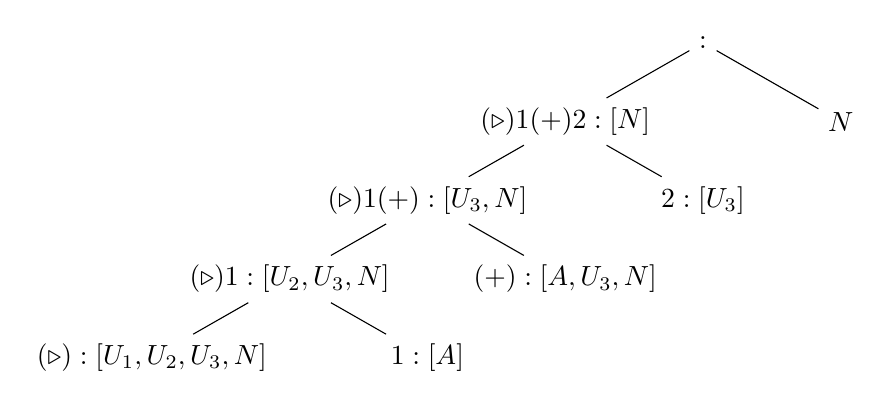
\begin{tikzpicture}
    \def\app{{\scriptsize app}}
    \def\f{{(\triangleright)}}
    \def\p{{(+)}}
    \node {:} [sibling distance = 3.5cm, level distance = 1cm]
        child {node {$\f 1 \p 2:[N]$}
            child {node {$\f 1 \p:[U_3, N]$}
                child {node {$\f 1:[U_2, U_3, N]$}
                    child {node {$\f: [U_1,U_2,U_3,N]$}}
                    child {node {$1: [A]$}}
                }
                child {node {$(+): [A,U_3,N]$}}
            }
            child {node {$2: [U_3]$}}
        }
        child {node {$N$}};
\end{tikzpicture}
}

We start with the elaboration of $(\triangleright) 1 (+) 2$ with the signature
requirement $[N]$ and the required type $N$.

\begin{itemize}
    \item The term is an application with the function term $(\triangleright) 1
        (+)$ and the argument $2$. We start the elaboration of the function term
        with the signature requirement $[U_3, N]$ and no required type.

    \item The term is again an application with the function term
        $(\triangleright) 1$ and the argument $(+)$. We start the elaboration
        of the function term with the signature requirement $[U_2, U_3, N]$ and
        no required type.

    \item The term is again an application with the function term
        $(\triangleright)$ and the argument $1$. We start the elaboration of the
        function term with the signature requirement $[U_1, U_2, U_3, N]$ and no
        required type.

    \item The term $(\triangleright)$ is a global name with the signature $[I,
        I, A, [A, P], P]$. Unification with the required signature $[U_1, U_2,
        U_3, N]$ results in
        $$
        \begin{array}{lll}
            U_1 &:=& A
            \\
            U_2 &:=& [A, U_3, N]
            \\
            P   &:=& [U_3, N]
        \end{array}
        $$
        Because of the two implicit arguments the term is elaborated as
        $(\triangleright)A P$ with the metavariables $A$ and $P$.

    \item Next the argument term $1$ has to be elaborated with the required
        signature $[A]$ and the required type $A$. This elaboration gets stuck
        on $A$, because the elaborator cannot decide the number type.

    \item Next the argument term $(+)$ is tried with the required signature $[A,
        U_3, N]$. The global name is ambiguous, but the ambiguity can be
        resolved by the result type. The signature is $[N, N, N]$. Unification
        with the required signature results in
        $$
        \begin{array}{lll}
            A &:=& N
            \\
            U_3 &:=& N
        \end{array}
        $$

    \item Now the complete term can be elaborated as
        $$
            (\triangleright) N (N \to N) \meta a (+) \meta b
        $$
        leaving the two holes $\meta a$ and $\meta b$ for the remaining
        arguments. However by unification the metavariables $\meta A$ and $\meta
        U_3$ are instantiated by $N$ and therefore the elaboration of the
        remaining arguments is unblocked and finally will succeed.
\end{itemize}


\section{Bound Variables}

The function type

$$
\Pi x^A. R
$$

has a bound variable $x$ of type $A$ and a result type $R$ which might depend on
$x$.

A bound variable has the following attributes.

\begin{enumerate}

    \item Implicit: Let $f: \Pi x^A. R$ be a function and $f a$ an application.
        If the bound variable is implicit, then the compiler is instructed to
        infer the argument $a$ from the context in case it is missing.

        Implicit arguments are always ghost arguments. No runtime decisions and
        not runtime objects can be constructed by using implicit arguments.

    \item Type relevant: A variable is type relevant if the result type depends
        on it.

        Open point: What happens in
        $$
            \Pi P^{A \to \Any} x^A. P x
        $$
        if $P = \lambda x^A . N$? Is $x$ type relevant?

    \item Ghost: A ghost variable means that its value cannot be used in the
        runtime code. It can be

        \begin{itemize}
            \item used in types

            \item used as an argument to a function which expects a ghost argument

            \item pattern matched on to make decisions if the result type of the
                decision is a proposition

            \item used as an argument to any function whose return type is a
                propositon.

        \end{itemize}
\end{enumerate}

A type is a proposition or a propositional type if its type is $\Prop$. All
other types are non propositional types. Any term whose type is a proposition is
a proof of the proposition. All terms whose type is a proposition are ghost
terms because they are never runtime objects.


There are the following rules:

\begin{enumerate}
    \item All type relevant arguments in a global function whose type is a
        proposition are mandatory implicit. If the function is not global, then
        the argument can be implicit or not.

    \item All type relevant arguments whose type is not a
        proposition can be declared implicit or not.

        If declared implicit, then they are ghost variables. This implies that
        the function is not allowed to make any runtime decisions or construct
        any runtime objects using the ghost argument. Ghost arguments are only
        available at compile time.

    \item If a non-ghost function is fed with a ghost argument where it expects
        a non-ghost argument (i.e. an explicit argument), then the result is
        infected i.e. the result is converted to a ghost object.

    \item An argument which is not type relevant is not allowed to be implicit.
\end{enumerate}


If a constructor for a proposition uses non-propositional bound variables, then the
non-propositonal bound variable is a ghost variable. A pattern match uncovering
it can use its value only as a ghost value. A decision cannot be made on pattern
match unless the result type of the pattern match is a proposition.


\section{Universes}





\subsection{Universes and Sorts}


We have the following sorts or universes (sorts and universes are synonymous):
\begin{enumerate}
\item $\Prop$: Impredicative universe of propositions

\item $\Any_i$: Predicative universes of types for $i \in \set{0, 1, 2, \ldots}$

\item $\Any_\infty$: Top universe
\end{enumerate}
and the builtin type $\Uni$ with the typing judgements which are treated as
axioms:
$$
\begin{array}{l}
    \Uni : \Any_\infty
    \\
    \Prop : \Any_0 : \Any_1 \ldots
\end{array}
$$


All sorts except the top sort $\Any_\infty$ have types. Therefore it is
possible to introduce type variables $X: s$ for all sorts except the top sort.

Furthermore since $\Uni$ has type $\Any_\infty$ it is possible to introduce
universe variables $u: \Uni$.

The type of a type is always a sort. The sort of a type defines the
universe of the type. I.e. all types live in a universe. The typing judgement
$T: s$ says that the type $T$ lives in the universe $s$.


There is a subtle difference between the universe of a type and the universe of
an object. An object has a type and its type lives in a universe. We say the an
\emph{object $o$ lives in a universe $s$ if its type $T$ lives in the universe
$s$}. I.e. the typing judgement $o : T : s$ must be valid. In other words $o$
has type $T$ and $T$ has type $s$.

A type $T$ can be regarded as a type. Then its type is a sort $s$ with $T : s$
and it therefore lives in the universe $s$ as a type.

However a type can be regarded as an object as well. Then there is the typing
judgement $T: s_1 : s_2$. We say the object $T$ lives in the universe $s_2$.

Some examples: The type $\Nat$ lives in the universe $\Any_0$. The object $1$
has type $\Nat$. Therefore the object $1$ lives in the universe $\Any_0$. The
object $\Nat$ has type $\Any_0$ which has the type $\Any_1$. Therefore the
object $\Nat$ lives in the universe $\Any_1$. By the same reasoning the object
$\Any_0$ lives in the universe $\Any_2$.

All types regarded as objects live in a universe higher than the types regarded
as types.


Typing rules for products:
$$
\begin{array}{lll}
    \rulev{
        \Gamma \vdash A: s
        \\
        \Gamma, x^A \vdash B: \Prop
        \\
        A \ne \Uni
    }
    {
        \Gamma \vdash \Pi x^A. B : \Prop
    }
    &
    \rulev{
        \Gamma \vdash A: \Any_i
        \\
        \Gamma, x^A \vdash B: \Any_i
        \\
        A \ne \Uni
    }
    {
        \Gamma \vdash \Pi x^A. B : \Any_i
    }
    &
    \rulev{
        \Gamma \vdash u: \Uni
        \\
        \Gamma, u^\Uni \vdash B: s
        \\
        A \ne \Uni
    }
    {
        \Gamma \vdash \Pi u^\Uni. B : \Any_\infty
    }
\end{array}
$$
These rules guarantee that the type $\Pi u^\infty. B$ of a universe polymorphic
object cannot be used as an argument to a function.


\section{Monads}





\subsection{Basics}
%--------------------------------------------------------------------------------




A monadic type is a type constructor with at least one type argument.
$$
    M: \Pi \Gamma A^\Any \Delta. \Any
$$

Type of a monadic bind operation:
$$
    \Pi A^\Any B^\Any \ldots \,.\,
    M \vec a A \vec b
    \to
    (A \to M \vec c B \vec d)
    \to
    M \vec e B \vec f
$$






\subsection{Recursion}
%--------------------------------------------------------------------------------

Form of monadic types where recursion is possible:

$$
\begin{array}{l}
    S \to R (D A) S
    \\
    S \to (D A \to S \to Z) \to Z
    \\
    S_1 \to \ldots \to S_n \to ((D A) \to S_1 \to \ldots \to S_n \to Z) \to Z
\end{array}
$$
where $D$ is an inductive type constructor with two constructors (one contains
$A$, the other not) and $R$ is an inductive record type constructor (only one
constructor.

Usually $D$ is either \lstinline!Maybe! or \lstinline!Result! and $R$ is a
tuple.
\begin{alba}
    S -> (Maybe A, S)

    S -> (Maybe A -> S -> Z) -> Z

    S1 -> S2 -> ... ->  (Maybe A -> S1 -> S2 -> ... -> Z) -> Z
\end{alba}




\subsection{Code Examples}
%--------------------------------------------------------------------------------




\paragraph{State with Success}

\ \begin{alba}
    State (A S: Any): Any :=
        S -> (Maybe A, S)

    return {A S: Any} (a: A): State A S :=
        \ s := (just a, s)

    (>>=) {A B S: Any} (m: State A S) (f: A -> State B S): State B S :=
        \ s1 :=
            match m s1 case
                \ (just a, s2) :=  (f a) s2     -- potential recursive call!
                \ (empty,  s2) :=  (empty, s2)
\end{alba}




\paragraph{Continuation with State and Success}

\ \begin{alba}
    Cont (S A R: Any): Any :=
        S -> ((Maybe A, S) -> R) -> R

    return {S A R: Any} (a: A): Cont S A R :=
        \ s k := k s (just a)

    (>>=) {S A B R: Any} (m: Cont S A R) (f: A -> Cont S B R): Cont S B R :=
        \ s kb :=
            m s1
              (case
                \ (just a, s2)  := f a s2 kb        -- potential recursive call
                \ (empty,  s2)  := kb (empty, s2))

    run {S A Any} (s: S) (m: Cont S (Maybe A) (Maybe A)): Maybe A :=
        m s (\ x := x)
\end{alba}







\paragraph{State}

\ \begin{alba}
    State (A S: Any): Any :=
        S -> (A, S)

    return {A S: Any} (a: A): State A S :=
        \ s := (a, s)

    (>>=) {A B S: Any} (m: State A S) (f: A -> State B S): State B S :=
        \ s :=
            match m s case
                \ (a, s2)  := f a s2

    map {A B S: Any} (f: A -> B) (m: State A S): State B S :=
            -- 'State' is covariant in 'A'
        \ s :=
            match m s case
                \ (a, s2) := (f a, s2)

    mapS {A S1 S2: Any} (f: S1 -> S2) (g: S2 -> S1) (m: State A S1): State A S2 :=
            -- 'State' is not variant in 'S'
        \ (s2: S2) :=
            match m (g s2)  case
                \ (a, s1) := (a, f s1)
\end{alba}




\paragraph{Continuation}

\ \begin{alba}
    Cont (A R: Any): Any :=
        (A -> R) -> R

    return {A R: Any} (a: A): Cont A R :=
        \ (k: A -> R) := k a

    (>>=) {A B R: Any} (m: Cont A R) (f: A -> Cont B R): Cont B R :=
        \ (k: B -> R) :=
            m (\ a := f a k)

    map {A B R: Any} (f: A -> B) (m: Cont A R): Cont B R :=
            -- 'Cont' is covariant in 'A'
        \ (k: B -> R) :=
            m (\ a := k (f a))

    mapR {A R1 R2: Any} (f: R2 -> R1) (m: Cont A R1): Cont A R2 :=
            -- 'Cont' is contravariant in 'R'
        \ (k: A -> R2) :=
            m (\ a :=  f (k a))


    run {A: Any} (m: Cont A A): A :=
        m (\ x := x)
\end{alba}




\paragraph{State with Continuation}

\ \begin{alba}
    SCont (S A R: Any): Any :=
        S -> (A -> S -> R) -> R
        -- or equivalent
        S -> ((A, S) -> R) -> R

    return {S A R: Any} (a: A): SCont S A R :=
        \ s k := k a s

    (>>=) {S A B R: Any} (m: SCont S A R) (f: A -> SCont S B R): SCont S B R :=
        \  s1 kb :=
            m s1 (\ a s2 := f a s2 kb)

    map {S A B R: Any} (f: A -> B) (m: SCont S A R): SCont S B R :=
            -- 'Cont' is covariant in 'A'
        \ s1 kb
            m s1 (\ a s2 := kb (f a) s2)
\end{alba}




\paragraph{Function}

\ \begin{alba}
    Fun (X A: Any): Any :=
        X -> A

    return {X A: Any} (a: A): Fun X A :=
        \ _ := a

    (>>=) {X A B: Any} (m: Fun X A) (f: A -> Fun X B): Fun X B :=
        \ x :=
            f (m x)

    map {X A B: Any} (f: A -> B) (m: Fun X A): Fun X B :=
            -- 'Fun' is covariant in the result type
        \ x := f (m x)

    mapX {X1 X2 A: Any} (f: X2 -> X1) (m: Fun X1 A): Fun X2 A :=
            -- 'Fun' is contravariant in the argument type
        \ (x: X2) :=
            m (f x)
\end{alba}


\end{document}
